\chapter*{ANEXO A: Resultados extendidos}
\label{ch:anexo}

En este capítulo se muestra el detalle numérico de las métricas componentes de $CMOPSO-CLAHE$. además de valores resultantes de las variables de decisión y tiempos de ejecución para las imágenes de prueba. para los resultados no dominados. Los tiempos de ejecución detallados corresponden a \texttt{time())} \cite{time}.

%Los resultados de este apartado son los promedios de los tiempos de ejecución. de los algoritmos \textit{Histogram Equalization} (HE). \textit{Multiscale Morphological Contrast Enhancement} (MMCE) y el algoritmo propuesto. para las 200 imágenes en escala de grises. Los algoritmos se implementaron con el framewok ImageJ y se hizo ejecutar 5 veces los experimentos. En la Tabla \ref{tabla22} se muestran los promedios de los tiempos de ejecución del algoritmo HE para las imágenes en escala de grises.

\section{Imagen de prueba \texttt{calhouse\_230.jpg}}

\scriptsize
\begin{longtable}{|c|c|c|c|c|c|c|c|}
% \centering
%\begin{tabular}
\hline
ID & $\mathscr{R}_x$ & $\mathscr{R}_y$ & $\mathscr{C}$ & $f_1(I.\vv{x})$ & $f_2(I.\vv{x})$ & $f_3(I.\vv{x})$ & $f_4(I.\vv{x})$ \\
0 & 23 & 2 & 0.0 & 0.0292377 & 0.425724 & 0.412724 & 0.426577 \\
1 & 20 & 2 & 0.0 & 0.030087 & 0.42386 & 0.410826 & 0.424771 \\
2 & 17 & 2 & 0.0 & 0.0318866 & 0.421223 & 0.40784 & 0.422096 \\
3 & 14 & 3 & 0.0 & 0.0322351 & 0.418567 & 0.405405 & 0.419644 \\
4 & 16 & 2 & 0.0 & 0.0325675 & 0.418894 & 0.405988 & 0.420157 \\
5 & 11 & 2 & 0.0 & 0.0340767 & 0.413031 & 0.399763 & 0.414117 \\
6 & 7 & 2 & 0.0 & 0.0365424 & 0.401675 & 0.388628 & 0.402692 \\
7 & 18 & 2 & 0.0 & 0.038238 & 0.41038 & 0.396594 & 0.414668 \\
8 & 9 & 2 & 0.0 & 0.0391212 & 0.410855 & 0.397602 & 0.411904 \\
9 & 13 & 2 & 0.0 & 0.0397372 & 0.406896 & 0.392824 & 0.411252 \\
10 & 9 & 3 & 0.0 & 0.0419288 & 0.406245 & 0.393219 & 0.407594 \\
11 & 9 & 2 & 0.0 & 0.0425715 & 0.394656 & 0.380667 & 0.39842 \\
12 & 7 & 2 & 0.0 & 0.0488863 & 0.389568 & 0.375398 & 0.392996 \\
13 & 6 & 2 & 0.0 & 0.0519342 & 0.389407 & 0.374979 & 0.392855 \\
14 & 5 & 2 & 0.0 & 0.0532846 & 0.383024 & 0.369461 & 0.383779 \\
15 & 5 & 2 & 0.0 & 0.0570464 & 0.38065 & 0.366103 & 0.383668 \\
16 & 4 & 2 & 0.0 & 0.0581956 & 0.370847 & 0.355854 & 0.372697 \\
17 & 2 & 4 & 0.0 & 0.0678334 & 0.332408 & 0.319416 & 0.329963 \\
18 & 2 & 3 & 0.0 & 0.083076 & 0.330307 & 0.315432 & 0.327533 \\
19 & 2 & 3 & 0.0 & 0.107766 & 0.300927 & 0.288565 & 0.302558 \\
20 & 2 & 2 & 0.0 & 0.130446 & 0.288674 & 0.274897 & 0.29182 \\
21 & 37 & 4 & 0.421103062234 & 0.388474 & 0.0796014 & 0.0715557 & 0.0737911 \\
22 & 44 & 3 & 0.177772531513 & 0.420316 & 0.0571285 & 0.0508797 & 0.0542069 \\
23 & 2 & 2 & 1.0 & 0.422673 & 0.0391384 & 0.0356485 & 0.0375976 \\
24 & 2 & 2 & 0.966457510597 & 0.441196 & 0.0358967 & 0.0326292 & 0.0344847 \\
25 & 2 & 2 & 0.909807336447 & 0.452317 & 0.0334806 & 0.0305298 & 0.0321478 \\
26 & 2 & 3 & 0.871347872644 & 0.460282 & 0.0313939 & 0.0285593 & 0.0301892 \\
27 & 2 & 3 & 0.838052371298 & 0.472741 & 0.0288693 & 0.0262626 & 0.0277464 \\
28 & 2 & 3 & 0.78970323092 & 0.483203 & 0.0264133 & 0.0241076 & 0.0254163 \\
29 & 2 & 3 & 0.763073541042 & 0.494502 & 0.0247892 & 0.0225578 & 0.0238702 \\
30 & 2 & 3 & 0.734387233109 & 0.505156 & 0.0216592 & 0.0196863 & 0.0208914 \\
31 & 2 & 2 & 0.689415824019 & 0.516532 & 0.0201843 & 0.0183705 & 0.0194163 \\
32 & 2 & 2 & 0.674049273864 & 0.530366 & 0.0177617 & 0.0161534 & 0.0170947 \\
33 & 2 & 2 & 0.620573402397 & 0.544854 & 0.0155038 & 0.0140995 & 0.0149364 \\
34 & 2 & 2 & 0.594946439658 & 0.567288 & 0.0141571 & 0.0127951 & 0.0135701 \\
35 & 2 & 3 & 0.525728438652 & 0.571877 & 0.0115625 & 0.0105159 & 0.011121 \\
36 & 2 & 2 & 0.5 & 0.588363 & 0.0108908 & 0.00987159 & 0.0104669 \\
37 & 2 & 3 & 0.483071040731 & 0.59779 & 0.00906811 & 0.00822819 & 0.00867055 \\
38 & 2 & 5 & 0.456916541899 & 0.611275 & 0.00897331 & 0.00823064 & 0.00851013 \\
39 & 2 & 2 & 0.428434700311 & 0.614437 & 0.00742514 & 0.00670994 & 0.00714773 \\
40 & 2 & 3 & 0.390144531289 & 0.628389 & 0.00650833 & 0.00588966 & 0.00621115 \\
41 & 2 & 4 & 0.38446541693 & 0.631133 & 0.00581047 & 0.00528148 & 0.00556787 \\
42 & 2 & 3 & 0.37527195105 & 0.64904 & 0.0048614 & 0.00438096 & 0.00457561 \\
43 & 2 & 3 & 0.31193055736 & 0.65892 & 0.00444588 & 0.0039587 & 0.00415919 \\
44 & 2 & 3 & 0.310920748974 & 0.667173 & 0.00401135 & 0.00358585 & 0.00381668 \\
45 & 2 & 4 & 0.290295960924 & 0.681955 & 0.00282212 & 0.002562 & 0.002621 \\
46 & 2 & 3 & 0.244028880272 & 0.698645 & 0.00224598 & 0.00200366 & 0.00205784 \\
47 & 2 & 3 & 0.198283113397 & 0.708029 & 0.00164594 & 0.0014135 & 0.00148235 \\
48 & 2 & 3 & 0.150847773862 & 0.721569 & 0.00132173 & 0.00109436 & 0.00111522 \\
49 & 2 & 5 & 0.161790895768 & 0.744286 & 0.00127126 & 0.00105903 & 0.00109671 \\
50 & 2 & 2 & 0.153546446329 & 0.744481 & 0.00108487 & 0.000878814 & 0.000907648 \\
51 & 3 & 3 & 0.145704588048 & 0.747523 & 0.00103455 & 0.000816322 & 0.000848165 \\
52 & 2 & 3 & 0.146162992336 & 0.753901 & 0.000827484 & 0.000614913 & 0.000645663 \\
53 & 2 & 2 & 0.112761751028 & 0.759912 & 0.000615229 & 0.00043859 & 0.000453515 \\
54 & 2 & 3 & 0.00011646417386 & 0.775049 & 0.000299272 & 0.000143607 & 0.000141378 \\
55 & 2 & 2 & 0.00178837395609 & 0.786418 & 0.000323289 & 0.000143135 & 0.000182232 \\
56 & 2 & 2 & 0.0281221731315 & 0.788927 & 0.000204143 & 5.26475e-05 & 5.18143e-05 \\
\hline
\multicolumn{8}{|c|}{\textbf{Tiempos de ejecución:} \texttt{real:70m10.567s.user:207m55.583s.sys:95m37.939s}}\\  \hline
% \end{tabular}
\caption{Resultados no dominados para la imagen de prueba \texttt{calhouse\_230.jpg}}
\label{tab:calhouse_230}
\end{longtable}
\normalsize

\begin{figure}[H]
\centering
    %\begin{subfigure}[t]{0.45\textwidth}
    \begin{subfigure}[ID=0]{
    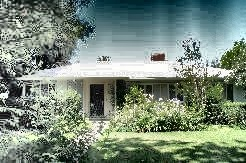
\includegraphics[width=0.45\textwidth]{./Figures/calhouse_230/0-resultado.jpg}
    }
%        \caption{Imagen Original. $\mathscr{H_Y}=0.207231$. $SSIM_R=1$. $SSIM_G=1$. $SSIM_B=1$}
\label{fig:calhouse2300}
\end{subfigure}
    ~ %add desired spacing between images. e. g. ~. \quad. \qquad. \hfill etc. 
      %(or a blank line to force the subfigure onto a new line)
      \begin{subfigure}[ID=1]{
      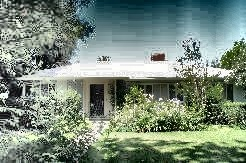
\includegraphics[width=0.45\textwidth]{./Figures/calhouse_230/1-resultado.jpg}   
      }
    %\begin{subfigure}[t]{0.45\textwidth}
%        \caption{Enhanced Image. $\mathscr{H_Y}=0.611275$. $SSIM_R=0.00897331$. $SSIM_G=0.00823064$. $SSIM_B=0.00851013$}
\label{fig:calhouse2301}
\end{subfigure}
    ~ %add desired spacing between images. e. g. ~. \quad. \qquad. \hfill etc. 
    %(or a blank line to force the subfigure onto a new line)
    \begin{subfigure}[ID=23]{
    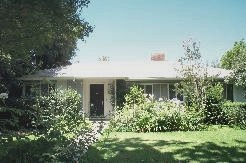
\includegraphics[width=0.45\textwidth]{./Figures/calhouse_230/23-resultado.jpg}
    }
    % \begin{subfigure}[t]{0.45\textwidth}
%        \caption{Enhanced Image.  $\mathscr{H_Y}=0.0350595$. $SSIM_R=0.416776$. $SSIM_G=0.403636$. $SSIM_B=0.417654$}
\label{fig:calhouse23023}
\end{subfigure} 
\begin{subfigure}[ID=24]{
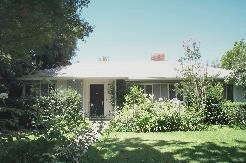
\includegraphics[width=0.45\textwidth]{./Figures/calhouse_230/24-resultado.jpg}
}
    % \begin{subfigure}[t]{0.45\textwidth}
        %\caption{Enhanced Image using \cite{morepso}. $\mathscr{H_Y}=0.788927$. $SSIM_R=0.000204143$. $SSIM_G=0.0000526475$. $SSIM_B=0.0000518143$}
        \label{fig:calhouse23024}
        \end{subfigure}
    ~ %add desired spacing between images. e. g. ~. \quad. \qquad. \hfill etc. 
    %(or a blank line to force the subfigure onto a new line)
    \begin{subfigure}[ID=56]{
    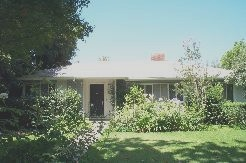
\includegraphics[width=0.45\textwidth]{./Figures/calhouse_230/56-resultado.jpg}
    }
    % \begin{subfigure}[t]{0.45\textwidth}
%        \caption{Enhanced Image.  $\mathscr{H_Y}=0.0350595$. $SSIM_R=0.416776$. $SSIM_G=0.403636$. $SSIM_B=0.417654$}
\label{fig:calhouse23056}
\end{subfigure} 
\begin{subfigure}[Imagen Original]{
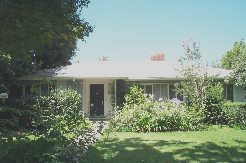
\includegraphics[width=0.45\textwidth]{./Figures/calhouse_230/calhouse_230.jpg}
}
    % \begin{subfigure}[t]{0.45\textwidth}
        %\caption{Enhanced Image using \cite{morepso}. $\mathscr{H_Y}=0.788927$. $SSIM_R=0.000204143$. $SSIM_G=0.0000526475$. $SSIM_B=0.0000518143$}
        \label{fig:calhouse230orig}
        \end{subfigure}
        \caption{Imágenes visualmente relevantes obtenidas mediante $CMOPSO-CLAHE$. Las variables y decisión y métricas de las imágenes se muestran en la tabla \ref{tab:calhouse_230}.}\label{fig:anexocalhouse230}
        \end{figure}

        \begin{figure}[H]
        \centering
        %\begin{subfigure}[Gráfica de Frente Pareto para las soluciones no dominadas de \texttt{calhouse_231.jpg}]{
        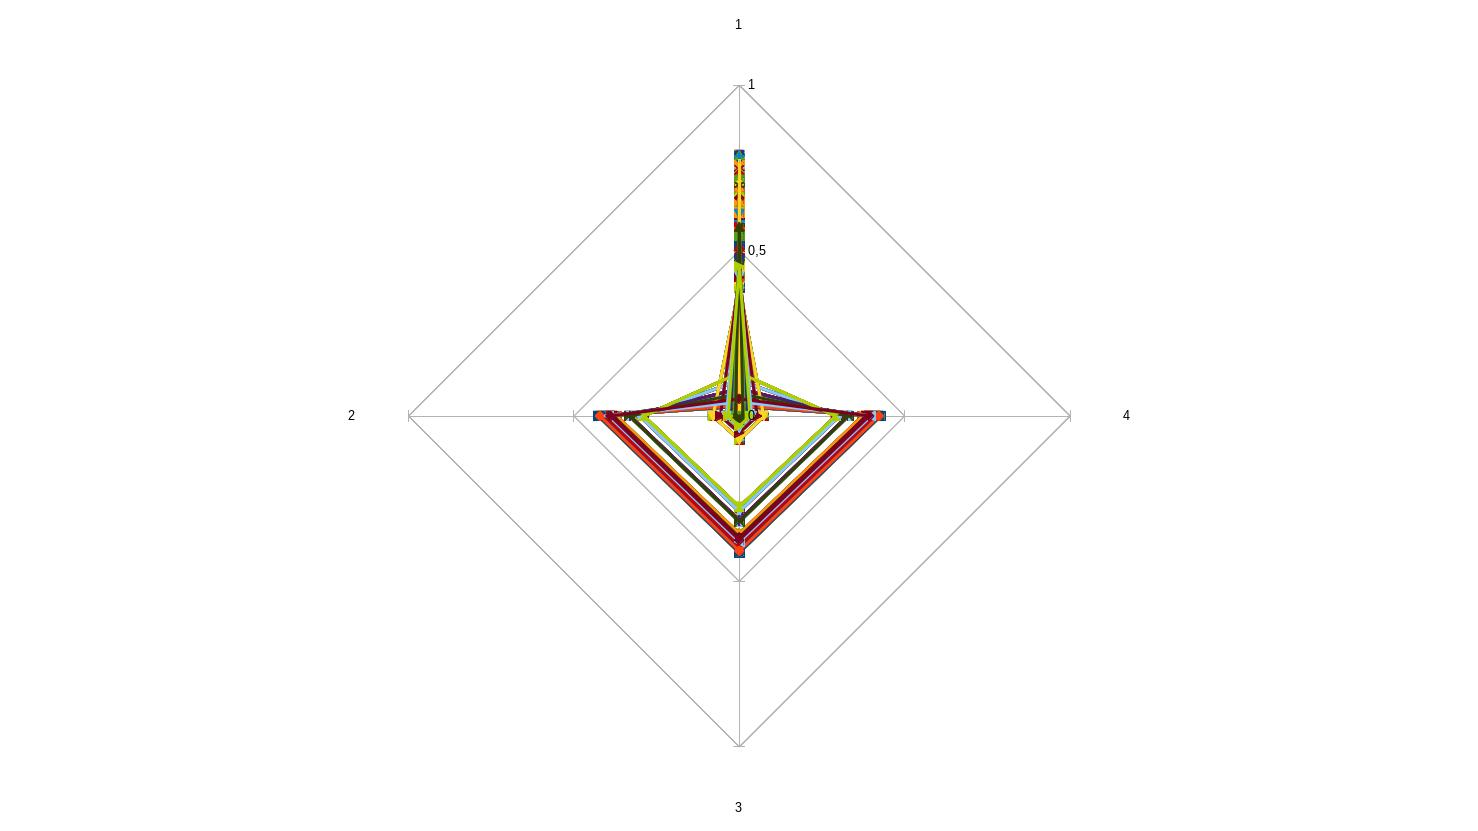
\includegraphics[width=\textwidth]{./Figures/calhouse_230/calhouse_230_2.jpg}
        %}
        %\end{subfigure}
        \caption{Frente pareto que contrasta los objetivos de las soluciones no dominadas. para los resultados de imágenes que se muestran en la tabla \ref{tab:calhouse_230}.}
        \label{fig:calhouse2302fp}
        \end{figure}


\section{Imagen de prueba \texttt{calhouse\_231.jpg}}

%calhouse 231
\scriptsize
\begin{longtable}{|c|c|c|c|c|c|c|c|}
% \centering
%\begin{tabular}
\hline
ID & $\mathscr{R}_x$ & $\mathscr{R}_y$ & $\mathscr{C}$ & $f_1(I.\vv{x})$ & $f_2(I.\vv{x})$ & $f_3(I.\vv{x})$ & $f_4(I.\vv{x})$ \\
0 & 18 & 3 & 0 & 0.00900173 & 0.267205 & 0.261971 & 0.266923 \\
1 & 13 & 2 & 0 & 0.00985956 & 0.259264 & 0.253973 & 0.258887 \\
2 & 10 & 2 & 0 & 0.00997639 & 0.256986 & 0.251503 & 0.256516 \\
3 & 10 & 2 & 0 & 0.0104213 & 0.255358 & 0.250056 & 0.255104 \\
4 & 8 & 2 & 0 & 0.0106044 & 0.253247 & 0.248009 & 0.252956 \\
5 & 8 & 2 & 0 & 0.0108852 & 0.248894 & 0.243521 & 0.248512 \\
6 & 5 & 3 & 0 & 0.0116286 & 0.242855 & 0.23726 & 0.242463 \\
7 & 37 & 2 & 0 & 0.0125856 & 0.204869 & 0.200071 & 0.20363 \\
8 & 18 & 2 & 0 & 0.012713 & 0.194229 & 0.189516 & 0.193111 \\
9 & 12 & 2 & 0 & 0.0130296 & 0.188019 & 0.183258 & 0.186758 \\
10 & 10 & 2 & 0 & 0.0133905 & 0.185665 & 0.180876 & 0.184348 \\
11 & 9 & 2 & 0 & 0.0134821 & 0.183211 & 0.178539 & 0.181995 \\
12 & 7 & 2 & 0 & 0.014287 & 0.177174 & 0.172057 & 0.1757 \\
13 & 5 & 2 & 0 & 0.0163016 & 0.174128 & 0.168903 & 0.172582 \\
14 & 4 & 2 & 0 & 0.0177784 & 0.168074 & 0.162957 & 0.166491 \\
15 & 3 & 2 & 0 & 0.0226231 & 0.1636 & 0.159053 & 0.162368 \\
16 & 2 & 2 & 0 & 0.026926 & 0.160205 & 0.156303 & 0.159384 \\
17 & 2 & 2 & 0 & 0.0431004 & 0.13865 & 0.136192 & 0.138648 \\
18 & 20 & 2 & 1 & 0.270889 & 0.0385879 & 0.0376327 & 0.0382134 \\
19 & 18 & 2 & 1 & 0.271006 & 0.0385725 & 0.0376188 & 0.0381991 \\
20 & 7 & 2 & 0.964079732103 & 0.276454 & 0.0381787 & 0.0368181 & 0.0376312 \\
21 & 2 & 2 & 0.989356928034 & 0.282013 & 0.038501 & 0.036779 & 0.0381451 \\
22 & 6 & 2 & 1 & 0.282743 & 0.0378731 & 0.0366182 & 0.0374679 \\
23 & 3 & 2 & 0.971840503575 & 0.284309 & 0.0371586 & 0.0357552 & 0.0367035 \\
24 & 4 & 2 & 0.972742419204 & 0.288689 & 0.0362972 & 0.0349026 & 0.0357714 \\
25 & 2 & 2 & 0.935457791487 & 0.289546 & 0.0364327 & 0.0347045 & 0.0360937 \\
26 & 2 & 2 & 0.940446088318 & 0.293769 & 0.0358847 & 0.0344679 & 0.0355097 \\
27 & 6 & 2 & 0.904740520538 & 0.295335 & 0.0347202 & 0.0334983 & 0.0342668 \\
28 & 9 & 2 & 1 & 0.298885 & 0.0334443 & 0.0324061 & 0.0330044 \\
29 & 14 & 2 & 1 & 0.299743 & 0.0334014 & 0.0323744 & 0.0329796 \\
30 & 10 & 2 & 0.913917022567 & 0.306106 & 0.0327387 & 0.0317938 & 0.032341 \\
31 & 12 & 2 & 1 & 0.307615 & 0.032043 & 0.0310592 & 0.0315852 \\
32 & 2 & 2 & 0.868629026061 & 0.309887 & 0.0325293 & 0.0309195 & 0.0322076 \\
33 & 7 & 2 & 0.922386499146 & 0.312944 & 0.0307703 & 0.0297033 & 0.0303923 \\
34 & 2 & 2 & 0.873918676927 & 0.314815 & 0.0305687 & 0.0293387 & 0.0302264 \\
35 & 12 & 2 & 0.828307512256 & 0.315595 & 0.029047 & 0.0281777 & 0.0286568 \\
36 & 7 & 2 & 0.90021573696 & 0.319267 & 0.0277445 & 0.0268512 & 0.0273699 \\
37 & 5 & 2 & 0.858598604984 & 0.325659 & 0.0279524 & 0.0268406 & 0.0275564 \\
38 & 6 & 2 & 0.856682527935 & 0.328166 & 0.0265695 & 0.0256397 & 0.0261868 \\
39 & 2 & 2 & 0.810611535096 & 0.333691 & 0.0265783 & 0.0254337 & 0.0262778 \\
40 & 14 & 2 & 0.826919288172 & 0.338436 & 0.0232717 & 0.0226148 & 0.0229894 \\
41 & 3 & 2 & 0.747934727522 & 0.354162 & 0.0228098 & 0.0218175 & 0.0225493 \\
42 & 2 & 2 & 0.715468922759 & 0.359465 & 0.0228153 & 0.0216203 & 0.0225292 \\
43 & 7 & 2 & 0.738152056945 & 0.362255 & 0.0220707 & 0.0212203 & 0.0216666 \\
44 & 5 & 2 & 0.710949498481 & 0.3623 & 0.0212484 & 0.0204049 & 0.0209322 \\
45 & 8 & 2 & 0.71860927648 & 0.365558 & 0.0191753 & 0.0185399 & 0.0188855 \\
46 & 17 & 2 & 0.638555526222 & 0.367131 & 0.0189012 & 0.0183635 & 0.0186746 \\
47 & 24 & 2 & 0.888901260944 & 0.372819 & 0.0186476 & 0.0180095 & 0.0183297 \\
48 & 7 & 2 & 0.643958573155 & 0.37555 & 0.0169599 & 0.0164014 & 0.016725 \\
49 & 5 & 2 & 0.627441542801 & 0.383322 & 0.0160663 & 0.0154653 & 0.0158211 \\
50 & 3 & 2 & 0.629994003473 & 0.391768 & 0.0161627 & 0.0153941 & 0.0159548 \\
51 & 19 & 2 & 0.545081379984 & 0.397269 & 0.0143794 & 0.0139211 & 0.0141685 \\
52 & 3 & 2 & 0.601135625969 & 0.402347 & 0.0145436 & 0.0138748 & 0.0143605 \\
53 & 3 & 2 & 0.57753934137 & 0.411112 & 0.013378 & 0.0127763 & 0.0131599 \\
54 & 2 & 2 & 0.541426023964 & 0.41398 & 0.0131499 & 0.0124833 & 0.0130018 \\
55 & 3 & 2 & 0.544335817577 & 0.414029 & 0.0125525 & 0.0119757 & 0.0123731 \\
56 & 6 & 2 & 0.548121706633 & 0.414094 & 0.0120755 & 0.0115387 & 0.0117838 \\
57 & 2 & 2 & 0.515852425305 & 0.421322 & 0.011292 & 0.010746 & 0.0111554 \\
58 & 31 & 2 & 0.0280991811699 & 0.423455 & 0.0107604 & 0.0102737 & 0.010496 \\
59 & 33 & 2 & 0.510626077249 & 0.42346 & 0.0107601 & 0.0102734 & 0.0104956 \\
60 & 3 & 2 & 0.5 & 0.426877 & 0.0107589 & 0.0102665 & 0.0106218 \\
61 & 9 & 2 & 0.5 & 0.428904 & 0.0107733 & 0.0101945 & 0.0103729 \\
62 & 13 & 2 & 0.5 & 0.431454 & 0.00965356 & 0.00927182 & 0.0094467 \\
63 & 7 & 2 & 0.478914771532 & 0.435993 & 0.00828631 & 0.00795353 & 0.00813127 \\
64 & 5 & 2 & 0.457071559114 & 0.442431 & 0.00817965 & 0.00780437 & 0.0080066 \\
65 & 2 & 2 & 0.429496349756 & 0.446127 & 0.00810596 & 0.00772429 & 0.00801587 \\
66 & 3 & 2 & 0.442489234125 & 0.447001 & 0.00778622 & 0.00745209 & 0.00769754 \\
67 & 9 & 2 & 0.456539353563 & 0.45027 & 0.00668378 & 0.00648114 & 0.00659949 \\
68 & 5 & 2 & 0.376465221858 & 0.456932 & 0.00627423 & 0.00605903 & 0.00619215 \\
69 & 8 & 2 & 0.461600206088 & 0.460667 & 0.00621708 & 0.00592585 & 0.00603826 \\
70 & 8 & 2 & 0.360353977865 & 0.462861 & 0.00579699 & 0.00562394 & 0.00572817 \\
71 & 2 & 5 & 0.411676225675 & 0.471886 & 0.00573421 & 0.00559339 & 0.0057057 \\
72 & 3 & 2 & 0.372641778915 & 0.475316 & 0.00536055 & 0.00515606 & 0.00529048 \\
73 & 8 & 2 & 0.399775248471 & 0.475386 & 0.00529207 & 0.00510996 & 0.00520481 \\
74 & 3 & 2 & 0.339070248196 & 0.47558 & 0.00452605 & 0.004307 & 0.00443858 \\
75 & 4 & 2 & 0.351684592681 & 0.479774 & 0.00435225 & 0.00410036 & 0.00418851 \\
76 & 4 & 2 & 0.349489075978 & 0.482928 & 0.00426761 & 0.00405113 & 0.00415045 \\
77 & 3 & 2 & 0.337330254689 & 0.488762 & 0.00401598 & 0.00385289 & 0.00397122 \\
78 & 2 & 2 & 0.30899847401 & 0.491558 & 0.00390371 & 0.00373161 & 0.00387131 \\
79 & 2 & 9 & 0.278605575898 & 0.49243 & 0.00331112 & 0.00334138 & 0.00338704 \\
80 & 2 & 2 & 0.309171129718 & 0.49718 & 0.00289651 & 0.00277638 & 0.00282767 \\
81 & 2 & 9 & 0.22375153796 & 0.499764 & 0.00285511 & 0.00284174 & 0.0028875 \\
82 & 3 & 2 & 0.300745369259 & 0.506126 & 0.00229212 & 0.00217746 & 0.00221458 \\
83 & 4 & 2 & 0.263406661906 & 0.506628 & 0.00222147 & 0.00211851 & 0.00215494 \\
84 & 2 & 2 & 0.251424143589 & 0.513605 & 0.00194255 & 0.00184685 & 0.00190236 \\
85 & 5 & 2 & 0.243696919714 & 0.514978 & 0.00176819 & 0.00169965 & 0.00173187 \\
86 & 4 & 2 & 0.209648277039 & 0.516483 & 0.00166633 & 0.0015921 & 0.00162961 \\
87 & 4 & 3 & 0.266234136177 & 0.520381 & 0.00166707 & 0.00158428 & 0.0016109 \\
88 & 2 & 4 & 0.248121384745 & 0.521675 & 0.00161956 & 0.00153988 & 0.00158018 \\
89 & 3 & 2 & 0.213491461803 & 0.525156 & 0.00144721 & 0.00138333 & 0.00141691 \\
90 & 2 & 2 & 0.191537420599 & 0.52922 & 0.00135061 & 0.00127997 & 0.00130769 \\
91 & 3 & 2 & 0.183704209136 & 0.530389 & 0.00119938 & 0.00115064 & 0.00116924 \\
92 & 2 & 3 & 0.178720787449 & 0.534519 & 0.00114637 & 0.00109067 & 0.00111032 \\
93 & 7 & 2 & 0.241533503656 & 0.536006 & 0.00110823 & 0.00103223 & 0.00105307 \\
94 & 2 & 2 & 0.167767741924 & 0.540966 & 0.000784735 & 0.000735661 & 0.000749385 \\
95 & 2 & 3 & 0.165303683073 & 0.546799 & 0.000724879 & 0.000653544 & 0.000674347 \\
96 & 2 & 2 & 0.14568920398 & 0.549775 & 0.00055956 & 0.00050608 & 0.000516374 \\
97 & 2 & 7 & 0.0971302704582 & 0.551463 & 0.0005087 & 0.000484928 & 0.000491999 \\
98 & 3 & 4 & 0.0169016006744 & 0.55715 & 0.000453264 & 0.000428699 & 0.000432725 \\
99 & 2 & 3 & 0.0764136259071 & 0.561146 & 0.000201883 & 0.000166411 & 0.000174052 \\
100 & 2 & 2 & 0.049662954082 & 0.565069 & 0.000189286 & 0.000165373 & 0.000167802 \\
101 & 3 & 3 & 0.0412250071562 & 0.573604 & 0.000167373 & 0.000136933 & 0.000144334 \\
102 & 2 & 2 & 0.0213381170565 & 0.573629 & 0.000103816 & 7.68E-05 & 7.86E-05 \\
\hline
\multicolumn{8}{|c|}{\textbf{Tiempos de ejecución:} \texttt{real:70m26.492s. user:209m3.921s. sys:95m37.357s}}\\  \hline
% \end{tabular}
\caption{Resultados no dominados para la imagen de prueba \texttt{calhouse\_231.jpg}}
\label{tab:calhouse_231}
\end{longtable}
\normalsize

\begin{figure}[H]
\centering
    %\begin{subfigure}[t]{0.45\textwidth}
    \begin{subfigure}[ID=0]{
    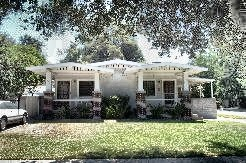
\includegraphics[width=0.45\textwidth]{./Figures/calhouse_231/0-resultado.jpg}
    }
%        \caption{Imagen Original. $\mathscr{H_Y}=0.207231$. $SSIM_R=1$. $SSIM_G=1$. $SSIM_B=1$}
\label{fig:calhouse2310}
\end{subfigure}
    ~ %add desired spacing between images. e. g. ~. \quad. \qquad. \hfill etc. 
      %(or a blank line to force the subfigure onto a new line)
      \begin{subfigure}[ID=1]{
      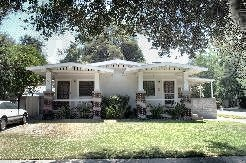
\includegraphics[width=0.45\textwidth]{./Figures/calhouse_231/1-resultado.jpg}   
      }
    %\begin{subfigure}[t]{0.45\textwidth}
%        \caption{Enhanced Image. $\mathscr{H_Y}=0.611275$. $SSIM_R=0.00897331$. $SSIM_G=0.00823064$. $SSIM_B=0.00851013$}
\label{fig:calhouse2311}
\end{subfigure}
    ~ %add desired spacing between images. e. g. ~. \quad. \qquad. \hfill etc. 
    %(or a blank line to force the subfigure onto a new line)
    \begin{subfigure}[ID=23]{
    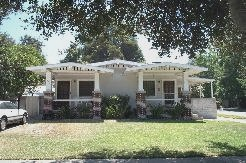
\includegraphics[width=0.45\textwidth]{./Figures/calhouse_231/28-resultado.jpg}
    }
    % \begin{subfigure}[t]{0.45\textwidth}
%        \caption{Enhanced Image.  $\mathscr{H_Y}=0.0350595$. $SSIM_R=0.416776$. $SSIM_G=0.403636$. $SSIM_B=0.417654$}
\label{fig:calhouse23128}
\end{subfigure} 
\begin{subfigure}[ID=24]{
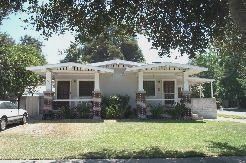
\includegraphics[width=0.45\textwidth]{./Figures/calhouse_231/29-resultado.jpg}
}
    % \begin{subfigure}[t]{0.45\textwidth}
        %\caption{Enhanced Image using \cite{morepso}. $\mathscr{H_Y}=0.788927$. $SSIM_R=0.000204143$. $SSIM_G=0.0000526475$. $SSIM_B=0.0000518143$}
        \label{fig:calhouse23129}
        \end{subfigure}
    ~ %add desired spacing between images. e. g. ~. \quad. \qquad. \hfill etc. 
    %(or a blank line to force the subfigure onto a new line)
    \begin{subfigure}[ID=56]{
    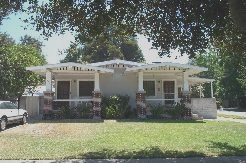
\includegraphics[width=0.45\textwidth]{./Figures/calhouse_231/102-resultado.jpg}
    }
    % \begin{subfigure}[t]{0.45\textwidth}
%        \caption{Enhanced Image.  $\mathscr{H_Y}=0.0350595$. $SSIM_R=0.416776$. $SSIM_G=0.403636$. $SSIM_B=0.417654$}
\label{fig:calhouse231102}
\end{subfigure} 
\begin{subfigure}[Imagen Original]{
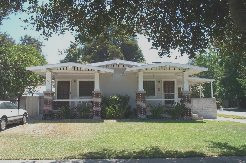
\includegraphics[width=0.45\textwidth]{./Figures/calhouse_231/calhouse_231.jpg}
}
    % \begin{subfigure}[t]{0.45\textwidth}
        %\caption{Enhanced Image using \cite{morepso}. $\mathscr{H_Y}=0.788927$. $SSIM_R=0.000204143$. $SSIM_G=0.0000526475$. $SSIM_B=0.0000518143$}
        \label{fig:calhouse231orig}
        \end{subfigure}
        \caption{Imágenes visualmente relevantes obtenidas mediante $CMOPSO-CLAHE$. Las variables y decisión y métricas de las imágenes se muestran en la tabla \ref{tab:calhouse_231}.}
        \label{fig:anexocalhouse230}
        \end{figure}

        \begin{figure}[H]
        \centering
        %\begin{subfigure}[Gráfica de Frente Pareto para las soluciones no dominadas de \texttt{calhouse_231.jpg}]{
        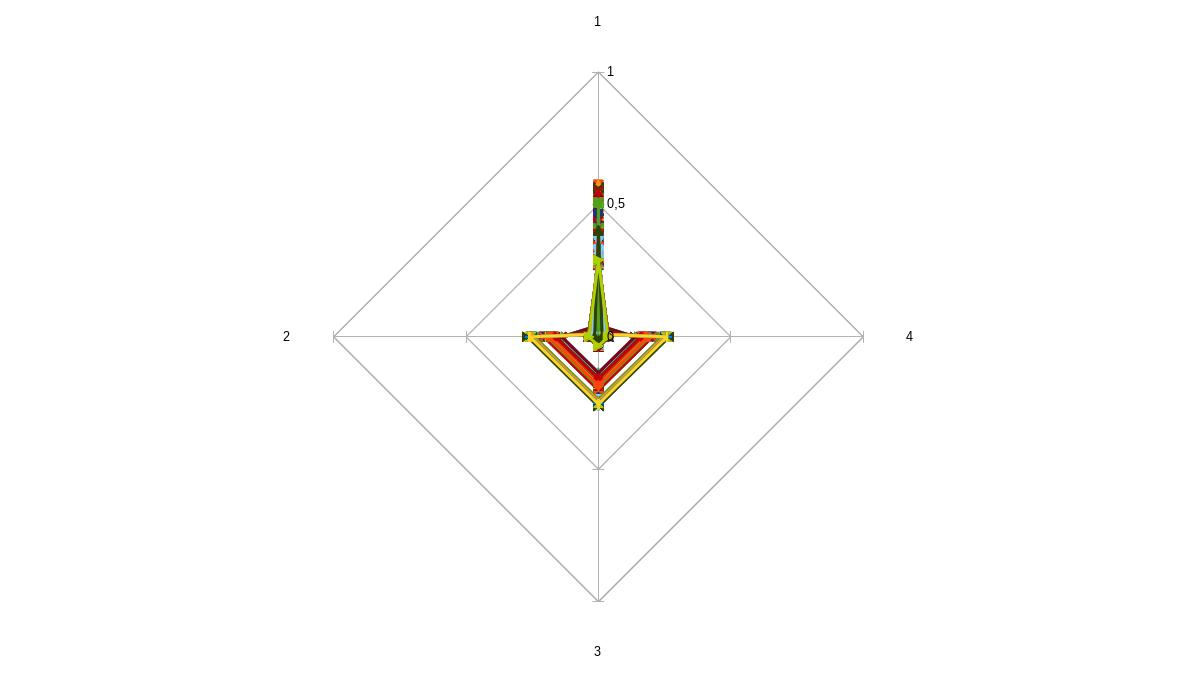
\includegraphics[width=\textwidth]{./Figures/calhouse_231/calhouse_231_2.jpg}
        %}
        %\end{subfigure}
        \caption{Frente pareto que contrasta los objetivos de las soluciones no dominadas. para los resultados de imágenes que se muestran en la tabla \ref{tab:calhouse_231}.}
        \label{fig:calhouse2312fp}
        \end{figure}

\section{Imagen de prueba \texttt{calhouse\_233.jpg}}

%calhouse 231
\scriptsize
\begin{longtable}{|c|c|c|c|c|c|c|c|}
% \centering
%\begin{tabular}
\hline
ID & $\mathscr{R}_x$ & $\mathscr{R}_y$ & $\mathscr{C}$ & $f_1(I.\vv{x})$ & $f_2(I.\vv{x})$ & $f_3(I.\vv{x})$ & $f_4(I.\vv{x})$ \\
0 & 4 & 2 & 0.0605454359216 & 1.08964 & 0.000295689 & 0.000153393 & 0.000162248 \\
1 & 2 & 3 & 0.0241100460642 & 1.05839 & 0.000302083 & 0.000187229 & 0.00018095 \\
2 & 3 & 2 & 0.0755634120675 & 1.08786 & 0.000329964 & 0.000184893 & 0.000199624 \\
3 & 2 & 6 & 0.0362807189867 & 1.03646 & 0.000641662 & 0.000514385 & 0.000524924 \\
4 & 8 & 3 & 0.103753483353 & 1.03239 & 0.00102858 & 0.000843436 & 0.000877847 \\
5 & 2 & 3 & 0.166601922869 & 0.993392 & 0.00117745 & 0.00100106 & 0.00102251 \\
6 & 4 & 3 & 0.197035454701 & 0.972543 & 0.00121931 & 0.00104515 & 0.00106603 \\
7 & 2 & 3 & 0.232499530296 & 0.95589 & 0.00235641 & 0.002009 & 0.00206351 \\
8 & 2 & 5 & 0.266574790017 & 0.938972 & 0.00280239 & 0.00262648 & 0.0026463 \\
9 & 2 & 3 & 0.278743476534 & 0.923925 & 0.00292607 & 0.00257795 & 0.00266449 \\
10 & 3 & 4 & 0.278646550346 & 0.92028 & 0.00292439 & 0.00261397 & 0.00266665 \\
11 & 12 & 3 & 0.30091560684 & 0.870766 & 0.00350392 & 0.00310311 & 0.00316902 \\
12 & 2 & 4 & 0.253592839376 & 0.919652 & 0.00348043 & 0.00316849 & 0.00322916 \\
13 & 2 & 3 & 0.391124890124 & 0.864988 & 0.00550206 & 0.00480986 & 0.00499557 \\
14 & 2 & 4 & 0.35510717405 & 0.830931 & 0.00598392 & 0.00560268 & 0.0056997 \\
15 & 16 & 3 & 0.227910808421 & 0.826457 & 0.00687623 & 0.00604448 & 0.00619402 \\
16 & 8 & 3 & 0.450962738883 & 0.819552 & 0.00842425 & 0.0076944 & 0.00785632 \\
17 & 5 & 3 & 0.5 & 0.810249 & 0.00887391 & 0.00800675 & 0.00821064 \\
18 & 2 & 3 & 0.534064898653 & 0.798087 & 0.0102274 & 0.00910215 & 0.00944354 \\
19 & 5 & 3 & 0.571647250785 & 0.785827 & 0.011758 & 0.0105297 & 0.010857 \\
20 & 2 & 4 & 0.506882563198 & 0.778071 & 0.0115198 & 0.0108465 & 0.0110746 \\
21 & 2 & 3 & 0.609611782643 & 0.763786 & 0.0131498 & 0.0117422 & 0.0121901 \\
22 & 3 & 4 & 0.590722339759 & 0.770255 & 0.0127545 & 0.0120351 & 0.0122763 \\
23 & 2 & 4 & 0.592771396022 & 0.759783 & 0.0134854 & 0.0128619 & 0.0130943 \\
24 & 10 & 3 & 0.569430012343 & 0.753103 & 0.0148294 & 0.0134841 & 0.0137764 \\
25 & 2 & 3 & 0.654795564549 & 0.758248 & 0.0146595 & 0.013324 & 0.0137805 \\
26 & 23 & 3 & 0.49018750213 & 0.745152 & 0.0156444 & 0.0140341 & 0.0143124 \\
27 & 5 & 3 & 0.711411054066 & 0.75186 & 0.0155433 & 0.0142944 & 0.0146168 \\
28 & 6 & 3 & 0.67594979599 & 0.742439 & 0.016272 & 0.014948 & 0.0152924 \\
29 & 3 & 3 & 0.697388429306 & 0.740592 & 0.0161852 & 0.0148598 & 0.015301 \\
30 & 2 & 4 & 0.619064681832 & 0.721047 & 0.0169986 & 0.0162408 & 0.0165372 \\
31 & 12 & 3 & 0.758015111952 & 0.715111 & 0.0179455 & 0.0167202 & 0.0170063 \\
32 & 2 & 4 & 0.664983118922 & 0.717893 & 0.018933 & 0.018076 & 0.0184091 \\
33 & 3 & 3 & 0.835945114263 & 0.715581 & 0.0212394 & 0.0197281 & 0.0202355 \\
34 & 18 & 4 & 0.235751993872 & 0.71698 & 0.0217524 & 0.0198408 & 0.0203643 \\
35 & 2 & 4 & 0.71221653662 & 0.697186 & 0.0211379 & 0.0202178 & 0.0205842 \\
36 & 3 & 3 & 0.841409534625 & 0.694649 & 0.024789 & 0.0230342 & 0.0236651 \\
37 & 2 & 4 & 0.775805262395 & 0.690287 & 0.0242775 & 0.023289 & 0.0236959 \\
38 & 6 & 3 & 0.946937444304 & 0.688181 & 0.027246 & 0.025366 & 0.0259008 \\
39 & 3 & 3 & 0.898145960419 & 0.688406 & 0.027186 & 0.0254119 & 0.0260424 \\
40 & 8 & 3 & 0.92952634183 & 0.682212 & 0.027619 & 0.026095 & 0.0265493 \\
41 & 2 & 3 & 0.92681679413 & 0.664923 & 0.0280842 & 0.0260755 & 0.0268696 \\
42 & 2 & 4 & 0.831514829931 & 0.682197 & 0.0278131 & 0.0267008 & 0.0271825 \\
43 & 3 & 3 & 1 & 0.662133 & 0.0302244 & 0.0283526 & 0.0290769 \\
44 & 2 & 3 & 1 & 0.638068 & 0.0319237 & 0.0297923 & 0.0307026 \\
45 & 44 & 3 & 0.340457573545 & 0.597537 & 0.0430642 & 0.0399363 & 0.0405722 \\
46 & 41 & 4 & 0.122685175212 & 0.585286 & 0.0791404 & 0.0724312 & 0.0744605 \\
47 & 2 & 2 & 0 & 0.166749 & 0.35221 & 0.33188 & 0.347256 \\
48 & 3 & 2 & 0 & 0.162343 & 0.36439 & 0.343949 & 0.35654 \\
49 & 4 & 2 & 0 & 0.0834117 & 0.383713 & 0.363361 & 0.373847 \\
50 & 5 & 2 & 0 & 0.0629735 & 0.391495 & 0.37163 & 0.381356 \\
51 & 11 & 2 & 0 & 0.0619745 & 0.418598 & 0.398414 & 0.406889 \\
52 & 26 & 2 & 0 & 0.0599365 & 0.437032 & 0.417224 & 0.424583 \\
53 & 6 & 3 & 0 & 0.0475216 & 0.459573 & 0.445796 & 0.456496 \\
54 & 9 & 3 & 0 & 0.0462856 & 0.470122 & 0.456474 & 0.466522 \\
55 & 11 & 3 & 0 & 0.0443048 & 0.475939 & 0.462247 & 0.471704 \\
56 & 2 & 6 & 0 & 0.0455046 & 0.470176 & 0.461747 & 0.47771 \\
57 & 2 & 7 & 0 & 0.0444002 & 0.493213 & 0.484229 & 0.499757 \\
58 & 2 & 9 & 0 & 0.0408697 & 0.499463 & 0.490757 & 0.507241 \\
59 & 2 & 10 & 0 & 0.0359039 & 0.511722 & 0.502448 & 0.518851 \\
60 & 2 & 2 & 0.00447401966895 & 1.09149 & 0.000183402 & 7.05E-05 & 6.21E-05 \\
\hline
\multicolumn{8}{|c|}{\textbf{Tiempos de ejecución:} \texttt{real:67m22.885s.user:207m13.352s.sys:94m57.439s
}}\\  \hline
% \end{tabular}
\caption{Resultados no dominados para la imagen de prueba \texttt{calhouse\_233.jpg}}
\label{tab:calhouse_233}
\end{longtable}
\normalsize

\begin{figure}[H]
\centering
    %\begin{subfigure}[t]{0.45\textwidth}
    \begin{subfigure}[ID=0]{
    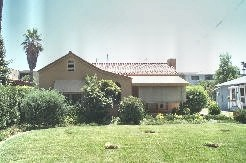
\includegraphics[width=0.45\textwidth]{./Figures/calhouse_233/6-resultado.jpg}
    }
%        \caption{Imagen Original. $\mathscr{H_Y}=0.207231$. $SSIM_R=1$. $SSIM_G=1$. $SSIM_B=1$}
\end{subfigure}
    ~ %add desired spacing between images. e. g. ~. \quad. \qquad. \hfill etc. 
      %(or a blank line to force the subfigure onto a new line)
      \begin{subfigure}[ID=1]{
      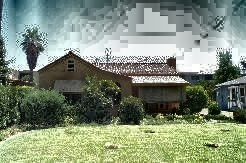
\includegraphics[width=0.45\textwidth]{./Figures/calhouse_233/7-resultado.jpg}   
      }
    %\begin{subfigure}[t]{0.45\textwidth}
%        \caption{Enhanced Image. $\mathscr{H_Y}=0.611275$. $SSIM_R=0.00897331$. $SSIM_G=0.00823064$. $SSIM_B=0.00851013$}
\end{subfigure}
    ~ %add desired spacing between images. e. g. ~. \quad. \qquad. \hfill etc. 
    %(or a blank line to force the subfigure onto a new line)
    \begin{subfigure}[ID=23]{
    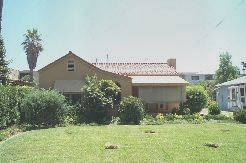
\includegraphics[width=0.45\textwidth]{./Figures/calhouse_233/46-resultado.jpg}
    }
    % \begin{subfigure}[t]{0.45\textwidth}
%        \caption{Enhanced Image.  $\mathscr{H_Y}=0.0350595$. $SSIM_R=0.416776$. $SSIM_G=0.403636$. $SSIM_B=0.417654$}
\end{subfigure} 
\begin{subfigure}[ID=24]{
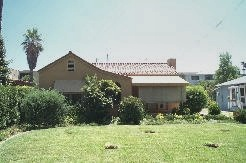
\includegraphics[width=0.45\textwidth]{./Figures/calhouse_233/47-resultado.jpg}
}
    % \begin{subfigure}[t]{0.45\textwidth}
        %\caption{Enhanced Image using \cite{morepso}. $\mathscr{H_Y}=0.788927$. $SSIM_R=0.000204143$. $SSIM_G=0.0000526475$. $SSIM_B=0.0000518143$}
        \label{fig:calhouse23129}
        \end{subfigure}
    ~ %add desired spacing between images. e. g. ~. \quad. \qquad. \hfill etc. 
    %(or a blank line to force the subfigure onto a new line)
    \begin{subfigure}[ID=56]{
    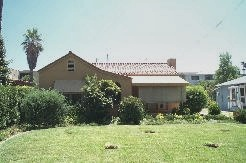
\includegraphics[width=0.45\textwidth]{./Figures/calhouse_233/60-resultado.jpg}
    }
    % \begin{subfigure}[t]{0.45\textwidth}
%        \caption{Enhanced Image.  $\mathscr{H_Y}=0.0350595$. $SSIM_R=0.416776$. $SSIM_G=0.403636$. $SSIM_B=0.417654$}
\label{fig:calhouse231102}
\end{subfigure} 
\begin{subfigure}[Imagen Original]{
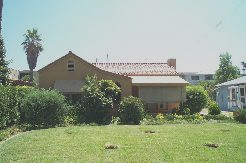
\includegraphics[width=0.45\textwidth]{./Figures/calhouse_233/calhouse_233.jpg}
}
    % \begin{subfigure}[t]{0.45\textwidth}
        %\caption{Enhanced Image using \cite{morepso}. $\mathscr{H_Y}=0.788927$. $SSIM_R=0.000204143$. $SSIM_G=0.0000526475$. $SSIM_B=0.0000518143$}
        \label{fig:calhouse233orig}
        \end{subfigure}
        \caption{Imágenes visualmente relevantes obtenidas mediante $CMOPSO-CLAHE$. Las variables y decisión y métricas de las imágenes se muestran en la tabla \ref{tab:calhouse_233}.}
        \label{fig:anexocalhouse233}
        \end{figure}

        \begin{figure}[H]
        \centering
        %\begin{subfigure}[Gráfica de Frente Pareto para las soluciones no dominadas de \texttt{calhouse_231.jpg}]{
        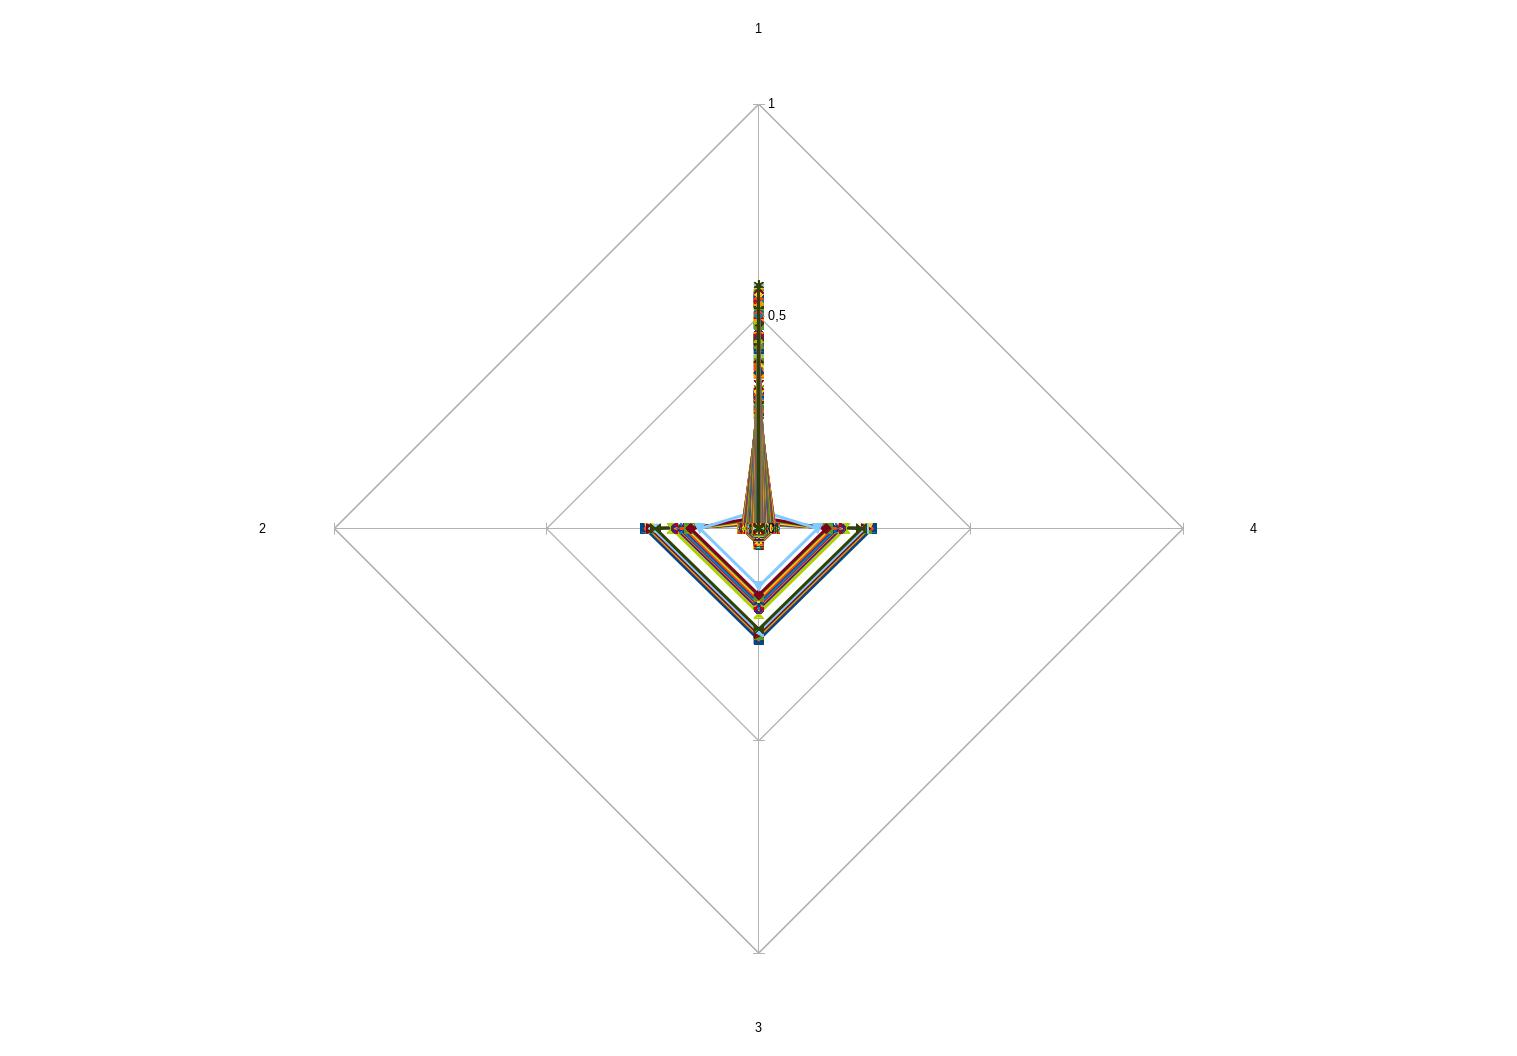
\includegraphics[width=\textwidth]{./Figures/calhouse_233/calhouse_233_2.jpg}
        %}
        %\end{subfigure}
        \caption{Frente pareto que contrasta los objetivos de las soluciones no dominadas. para los resultados de imágenes que se muestran en la tabla \ref{tab:calhouse_233}.}
        \label{fig:calhouse2332fp}
        \end{figure}


\section{Imagen de prueba \texttt{calhouse\_234.jpg}}

%calhouse 234
\scriptsize
\begin{longtable}{|c|c|c|c|c|c|c|c|}
% \centering
%\begin{tabular}
\hline
ID & $\mathscr{R}_x$ & $\mathscr{R}_y$ & $\mathscr{C}$ & $f_1(I.\vv{x})$ & $f_2(I.\vv{x})$ & $f_3(I.\vv{x})$ & $f_4(I.\vv{x})$ \\
2979 & 3 & 3 & 0.812519298752 & 0.511109 & 0.0287218 & 0.0274117 & 0.0284403 \\
2980 & 4 & 12 & 0 & 0.0276203 & 0.49051 & 0.486184 & 0.493034 \\
3091 & 4 & 2 & 0.853706507459 & 0.519737 & 0.027535 & 0.0255765 & 0.0267492 \\
3097 & 11 & 2 & 1 & 0.494054 & 0.034029 & 0.032038 & 0.0331011 \\
3104 & 20 & 3 & 0 & 0.0284328 & 0.402012 & 0.396043 & 0.401629 \\
3123 & 3 & 3 & 0.739306706876 & 0.533226 & 0.024867 & 0.0237548 & 0.0245899 \\
3125 & 2 & 2 & 0.731703535828 & 0.548753 & 0.0229975 & 0.0211807 & 0.0222653 \\
3126 & 3 & 2 & 0.679146848174 & 0.557746 & 0.0203147 & 0.0187927 & 0.0196922 \\
3127 & 2 & 2 & 0.850344549266 & 0.515146 & 0.029663 & 0.0272264 & 0.0286435 \\
3128 & 14 & 2 & 0.632770576643 & 0.58597 & 0.01286 & 0.0122675 & 0.0126854 \\
3129 & 53 & 3 & 0.0906614748552 & 0.41236 & 0.10348 & 0.0946411 & 0.0973958 \\
3130 & 8 & 2 & 0.368264089891 & 0.675727 & 0.00441494 & 0.00421142 & 0.00434589 \\
3131 & 2 & 2 & 0.827779089761 & 0.524632 & 0.0281598 & 0.0258405 & 0.0271833 \\
3132 & 2 & 2 & 0 & 0.138669 & 0.231124 & 0.221532 & 0.228493 \\
3133 & 37 & 4 & 0.488860216273 & 0.445821 & 0.0866204 & 0.0792098 & 0.0816776 \\
3134 & 4 & 2 & 0.255668440752 & 0.730788 & 0.00268251 & 0.00253008 & 0.00260924 \\
3135 & 6 & 2 & 0.912272466777 & 0.496642 & 0.0326795 & 0.0303633 & 0.0316357 \\
3136 & 2 & 2 & 0.0083970078807 & 0.835548 & 0.000142314 & 0.000115598 & 0.000110237 \\
3137 & 3 & 2 & 0.461160630083 & 0.650707 & 0.00852852 & 0.00796836 & 0.00830184 \\
3138 & 3 & 2 & 0.73164070769 & 0.551425 & 0.0215359 & 0.0198995 & 0.0208231 \\
3139 & 4 & 2 & 0.0653533397144 & 0.832464 & 0.000183395 & 0.000143403 & 0.000147903 \\
3140 & 3 & 2 & 0.148486630518 & 0.793742 & 0.000731432 & 0.000664557 & 0.000679274 \\
3141 & 18 & 2 & 0.572302594831 & 0.62303 & 0.00889421 & 0.00828233 & 0.00854233 \\
3142 & 13 & 3 & 0 & 0.0292034 & 0.390222 & 0.383769 & 0.389344 \\
3143 & 9 & 2 & 0.515175605936 & 0.640419 & 0.00871692 & 0.00817691 & 0.00844283 \\
3144 & 10 & 2 & 0.645449480383 & 0.580588 & 0.0168114 & 0.0159317 & 0.0165228 \\
3145 & 24 & 3 & 0 & 0.0277634 & 0.406696 & 0.400567 & 0.40603 \\
3146 & 6 & 2 & 0 & 0.0493283 & 0.277246 & 0.269315 & 0.27368 \\
3147 & 2 & 2 & 0.761261125963 & 0.54257 & 0.0246297 & 0.0226156 & 0.0237819 \\
3148 & 5 & 2 & 0 & 0.0519104 & 0.273498 & 0.265907 & 0.270653 \\
3149 & 2 & 2 & 0.926215684557 & 0.493326 & 0.0350073 & 0.032038 & 0.0337141 \\
3150 & 5 & 3 & 0.907757451731 & 0.507807 & 0.0309136 & 0.0296258 & 0.0305795 \\
3151 & 2 & 2 & 0.729074889936 & 0.553606 & 0.021385 & 0.0196689 & 0.0206698 \\
3152 & 3 & 2 & 0 & 0.0846047 & 0.245215 & 0.237309 & 0.244065 \\
3153 & 3 & 2 & 0.854113478667 & 0.512472 & 0.030045 & 0.027703 & 0.0290506 \\
3154 & 7 & 3 & 0 & 0.0321503 & 0.363205 & 0.357271 & 0.362161 \\
3155 & 24 & 2 & 1 & 0.448877 & 0.0337654 & 0.0325268 & 0.0334449 \\
3156 & 4 & 2 & 0.780918170773 & 0.530471 & 0.0249754 & 0.0230687 & 0.0241613 \\
3157 & 6 & 2 & 0.196390542599 & 0.78611 & 0.000841764 & 0.00080091 & 0.000816869 \\
3158 & 2 & 3 & 0.833866902733 & 0.511989 & 0.0302699 & 0.0285167 & 0.0297871 \\
3159 & 6 & 2 & 0.747192629244 & 0.547824 & 0.0229913 & 0.0213657 & 0.0222196 \\
3160 & 3 & 2 & 0.80975515976 & 0.527355 & 0.0266691 & 0.0245697 & 0.0257519 \\
3161 & 7 & 2 & 0 & 0.0413656 & 0.289774 & 0.282049 & 0.285934 \\
3162 & 3 & 3 & 0.725942475481 & 0.553035 & 0.0211689 & 0.0201818 & 0.0209119 \\
3163 & 2 & 3 & 0.0869925259854 & 0.831217 & 0.000254231 & 0.000202246 & 0.000220666 \\
3164 & 3 & 2 & 0.101165992212 & 0.829471 & 0.000258416 & 0.000220973 & 0.000231715 \\
3165 & 6 & 2 & 0.846937821181 & 0.518807 & 0.027765 & 0.0259249 & 0.0270216 \\
3166 & 3 & 2 & 0.305290000047 & 0.710093 & 0.00364066 & 0.0034385 & 0.00355669 \\
3167 & 11 & 2 & 0 & 0.0396638 & 0.306313 & 0.297956 & 0.302221 \\
3168 & 7 & 2 & 0.219179192327 & 0.773407 & 0.00121588 & 0.00114323 & 0.00117378 \\
3169 & 5 & 2 & 0.227660930211 & 0.738358 & 0.00171736 & 0.0016441 & 0.00168794 \\
3170 & 26 & 6 & 0.511796994819 & 0.445776 & 0.0921568 & 0.0871899 & 0.0896835 \\
3171 & 3 & 2 & 0.225128485738 & 0.755389 & 0.00142469 & 0.00136878 & 0.00139945 \\
3172 & 2 & 3 & 0.0112353502775 & 0.836594 & 0.000146742 & 0.000117982 & 0.000110062 \\
3173 & 17 & 2 & 0.73226869704 & 0.574325 & 0.0167192 & 0.0159348 & 0.0164249 \\
3174 & 11 & 3 & 0 & 0.0296307 & 0.381211 & 0.374829 & 0.380207 \\
3175 & 4 & 2 & 0.863033788718 & 0.502655 & 0.0311266 & 0.0287067 & 0.03005 \\
3176 & 14 & 2 & 0.937018260677 & 0.502234 & 0.0314391 & 0.0298899 & 0.0308901 \\
3177 & 3 & 3 & 0.578272628825 & 0.582351 & 0.0151525 & 0.0144716 & 0.0149766 \\
3178 & 6 & 2 & 0.682234104882 & 0.564373 & 0.0195332 & 0.0183163 & 0.019096 \\
3179 & 18 & 2 & 0.783902002406 & 0.533793 & 0.0238637 & 0.022623 & 0.0232914 \\
3180 & 4 & 3 & 0.403556720027 & 0.65922 & 0.00689137 & 0.00665012 & 0.00686885 \\
3181 & 2 & 3 & 0.885217278433 & 0.492458 & 0.0341363 & 0.0321934 & 0.0336531 \\
3182 & 11 & 2 & 0.317936251338 & 0.723333 & 0.00331185 & 0.00315496 & 0.00324682 \\
3183 & 15 & 2 & 0.5 & 0.666303 & 0.00554846 & 0.00524035 & 0.00540413 \\
3184 & 12 & 2 & 0.522610271857 & 0.601996 & 0.0103419 & 0.00983332 & 0.010186 \\
3185 & 11 & 2 & 0.95 & 0.513048 & 0.0288726 & 0.0272513 & 0.0282724 \\
3186 & 3 & 3 & 0.656165744218 & 0.571977 & 0.0180757 & 0.0172713 & 0.0179017 \\
3187 & 13 & 2 & 0.956428228721 & 0.524695 & 0.0260812 & 0.024745 & 0.0255167 \\
\hline
\multicolumn{8}{|c|}{\textbf{Tiempos de ejecución:} \texttt{real:69m51.735s, user:207m51.484s, sys:94m33.030s}}\\  \hline
% \end{tabular}
\caption{Resultados no dominados para la imagen de prueba \texttt{calhouse\_234.jpg}}
\label{tab:calhouse_234}
\end{longtable}
\normalsize

\begin{figure}[H]
\centering
    %\begin{subfigure}[t]{0.45\textwidth}
    \begin{subfigure}[ID=0]{
    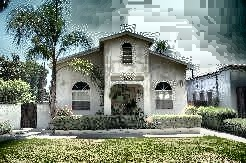
\includegraphics[width=0.45\textwidth]{./Figures/calhouse_234/1-resultado.jpg}
    }
%        \caption{Imagen Original. $\mathscr{H_Y}=0.207231$. $SSIM_R=1$. $SSIM_G=1$. $SSIM_B=1$}
\end{subfigure}
    ~ %add desired spacing between images. e. g. ~. \quad. \qquad. \hfill etc. 
      %(or a blank line to force the subfigure onto a new line)
      \begin{subfigure}[ID=1]{
      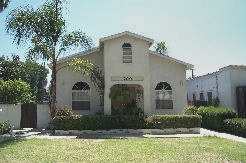
\includegraphics[width=0.45\textwidth]{./Figures/calhouse_234/2-resultado.jpg}   
      }
    %\begin{subfigure}[t]{0.45\textwidth}
%        \caption{Enhanced Image. $\mathscr{H_Y}=0.611275$. $SSIM_R=0.00897331$. $SSIM_G=0.00823064$. $SSIM_B=0.00851013$}
\end{subfigure}
    ~ %add desired spacing between images. e. g. ~. \quad. \qquad. \hfill etc. 
    %(or a blank line to force the subfigure onto a new line)
    \begin{subfigure}[ID=23]{
    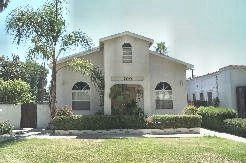
\includegraphics[width=0.45\textwidth]{./Figures/calhouse_234/51-resultado.jpg}
    }
    % \begin{subfigure}[t]{0.45\textwidth}
%        \caption{Enhanced Image.  $\mathscr{H_Y}=0.0350595$. $SSIM_R=0.416776$. $SSIM_G=0.403636$. $SSIM_B=0.417654$}
\end{subfigure} 
\begin{subfigure}[ID=24]{
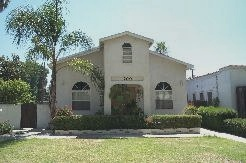
\includegraphics[width=0.45\textwidth]{./Figures/calhouse_234/59-resultado.jpg}
}
    % \begin{subfigure}[t]{0.45\textwidth}
        %\caption{Enhanced Image using \cite{morepso}. $\mathscr{H_Y}=0.788927$. $SSIM_R=0.000204143$. $SSIM_G=0.0000526475$. $SSIM_B=0.0000518143$}
        % \label{fig:calhouse23129}
        \end{subfigure}
    ~ %add desired spacing between images. e. g. ~. \quad. \qquad. \hfill etc. 
    %(or a blank line to force the subfigure onto a new line)
    \begin{subfigure}[ID=56]{
    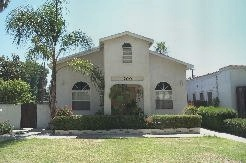
\includegraphics[width=0.45\textwidth]{./Figures/calhouse_234/60-resultado.jpg}
    }
    % \begin{subfigure}[t]{0.45\textwidth}
%        \caption{Enhanced Image.  $\mathscr{H_Y}=0.0350595$. $SSIM_R=0.416776$. $SSIM_G=0.403636$. $SSIM_B=0.417654$}
% \label{fig:calhouse231102}
\end{subfigure} 
\begin{subfigure}[Imagen Original]{
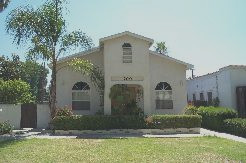
\includegraphics[width=0.45\textwidth]{./Figures/calhouse_234/calhouse_234.jpg}
}
    % \begin{subfigure}[t]{0.45\textwidth}
        %\caption{Enhanced Image using \cite{morepso}. $\mathscr{H_Y}=0.788927$. $SSIM_R=0.000204143$. $SSIM_G=0.0000526475$. $SSIM_B=0.0000518143$}
        % \label{fig:calhouse233orig}
        \end{subfigure}
        \caption{Imágenes visualmente relevantes obtenidas mediante $CMOPSO-CLAHE$. Las variables y decisión y métricas de las imágenes se muestran en la tabla \ref{tab:calhouse_234}.}
        \label{fig:anexocalhouse234}
        \end{figure}

        \begin{figure}[H]
        \centering
        %\begin{subfigure}[Gráfica de Frente Pareto para las soluciones no dominadas de \texttt{calhouse_231.jpg}]{
        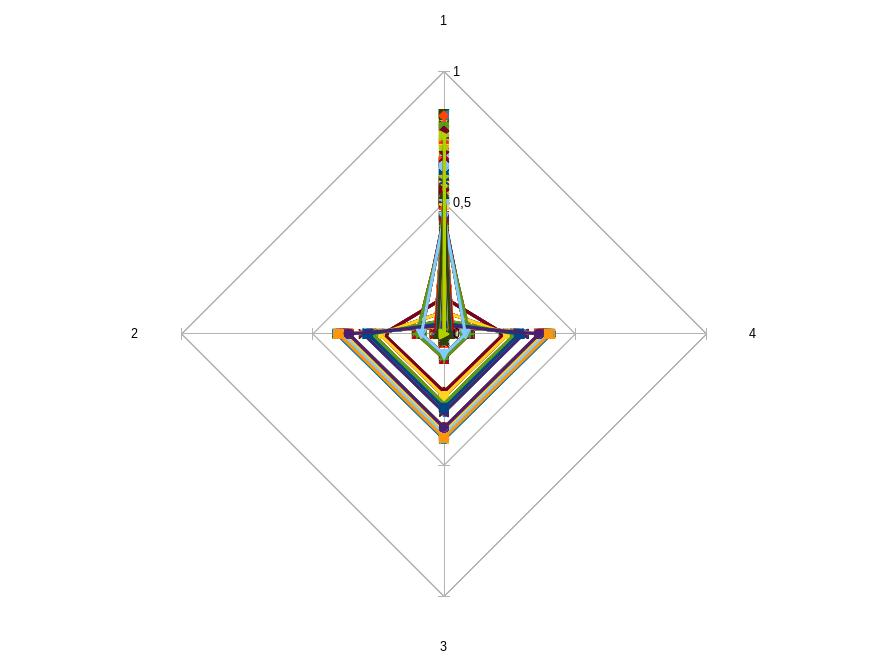
\includegraphics[width=\textwidth]{./Figures/calhouse_234/calhouse_234_2.jpg}
        %}
        %\end{subfigure}
        \caption{Frente pareto que contrasta los objetivos de las soluciones no dominadas. para los resultados de imágenes que se muestran en la tabla \ref{tab:calhouse_234}.}
        \label{fig:calhouse2342fp}
        \end{figure}


\section{Imagen de prueba \texttt{calhouse\_236.jpg}}

%calhouse 234
\scriptsize
\begin{longtable}{|c|c|c|c|c|c|c|c|}
% \centering
%\begin{tabular}
\hline
ID & $\mathscr{R}_x$ & $\mathscr{R}_y$ & $\mathscr{C}$ & $f_1(I.\vv{x})$ & $f_2(I.\vv{x})$ & $f_3(I.\vv{x})$ & $f_4(I.\vv{x})$ \\
\hline
9999 & 22 & 7 & 0.05 & 0.322022 & 0.106831 & 0.102759 & 0.104597 \\
7728 & 14 & 2 & 0.632770576643 & 0.58597 & 0.01286 & 0.0122675 & 0.0126854 \\
7730 & 8 & 2 & 0.368264089891 & 0.675727 & 0.00441494 & 0.00421142 & 0.00434589 \\
7732 & 2 & 2 & 0 & 0.138669 & 0.231124 & 0.221532 & 0.228493 \\
7736 & 2 & 2 & 0.0083970078807 & 0.835548 & 0.000142314 & 0.000115598 & 0.000110237 \\
7741 & 18 & 2 & 0.572302594831 & 0.62303 & 0.00889421 & 0.00828233 & 0.00854233 \\
7746 & 6 & 2 & 0 & 0.0493283 & 0.277246 & 0.269315 & 0.27368 \\
7748 & 5 & 2 & 0 & 0.0519104 & 0.273498 & 0.265907 & 0.270653 \\
7752 & 3 & 2 & 0 & 0.0846047 & 0.245215 & 0.237309 & 0.244065 \\
7755 & 24 & 2 & 1 & 0.448877 & 0.0337654 & 0.0325268 & 0.0334449 \\
7761 & 7 & 2 & 0 & 0.0413656 & 0.289774 & 0.282049 & 0.285934 \\
7772 & 2 & 3 & 0.0112353502775 & 0.836594 & 0.000146742 & 0.000117982 & 0.000110062 \\
7783 & 15 & 2 & 0.5 & 0.666303 & 0.00554846 & 0.00524035 & 0.00540413 \\
7784 & 12 & 2 & 0.522610271857 & 0.601996 & 0.0103419 & 0.00983332 & 0.010186 \\
7867 & 3 & 2 & 0.237164606413 & 0.699975 & 0.00309802 & 0.00307773 & 0.00326212 \\
7881 & 6 & 2 & 0 & 0.0297699 & 0.316537 & 0.313988 & 0.319524 \\
7882 & 41 & 4 & 0.277948416984 & 0.297561 & 0.107656 & 0.103902 & 0.105838 \\
7883 & 28 & 2 & 0 & 0.0209365 & 0.359519 & 0.358839 & 0.365177 \\
7884 & 7 & 2 & 0.5 & 0.596471 & 0.0133184 & 0.013128 & 0.0137713 \\
7885 & 2 & 2 & 0.0720277391995 & 0.787766 & 0.000256124 & 0.000197123 & 0.000228562 \\
7886 & 2 & 2 & 0.130899175101 & 0.758529 & 0.000769288 & 0.000722369 & 0.000767623 \\
7887 & 60 & 3 & 0.874629792235 & 0.276232 & 0.127112 & 0.120837 & 0.125981 \\
7888 & 2 & 2 & 0.80782701177 & 0.449825 & 0.0362412 & 0.0352132 & 0.0377132 \\
7889 & 4 & 2 & 0.211300785921 & 0.71229 & 0.00263194 & 0.00250156 & 0.00264687 \\
7890 & 14 & 2 & 0 & 0.0210977 & 0.346013 & 0.344528 & 0.350455 \\
7891 & 11 & 2 & 0 & 0.0218916 & 0.338454 & 0.336511 & 0.342515 \\
7892 & 18 & 2 & 0.0682579288587 & 0.677333 & 0.00469509 & 0.00463112 & 0.00484218 \\
7893 & 2 & 2 & 0.0997957374995 & 0.775215 & 0.000484727 & 0.000458843 & 0.000490921 \\
7894 & 2 & 2 & 0.018919608823 & 0.791656 & 0.000155317 & 0.000121572 & 0.000128309 \\
7895 & 2 & 2 & 0.307331880626 & 0.676598 & 0.00467596 & 0.00454571 & 0.00490102 \\
7896 & 2 & 2 & 0.220842134654 & 0.724546 & 0.00201504 & 0.00198291 & 0.00209202 \\
7897 & 2 & 2 & 0.954632188931 & 0.407068 & 0.0475321 & 0.0460638 & 0.0492886 \\
7898 & 2 & 2 & 0 & 0.0819087 & 0.255368 & 0.251915 & 0.257656 \\
7899 & 8 & 2 & 0 & 0.0249429 & 0.328823 & 0.326689 & 0.332172 \\
7900 & 2 & 2 & 0.179918780839 & 0.728299 & 0.00148275 & 0.00144158 & 0.00152957 \\
7901 & 2 & 2 & 0.554203660039 & 0.566152 & 0.0173144 & 0.0169155 & 0.0180509 \\
7902 & 12 & 2 & 0 & 0.0213795 & 0.343065 & 0.341144 & 0.347002 \\
7903 & 3 & 2 & 0.5 & 0.578231 & 0.0139116 & 0.0136808 & 0.0144633 \\
7904 & 3 & 2 & 0.0706628169375 & 0.780215 & 0.0003251 & 0.000293507 & 0.000313995 \\
7905 & 28 & 5 & 0.667890089724 & 0.330317 & 0.0943822 & 0.0913762 & 0.0924006 \\
7906 & 2 & 2 & 0.123897192018 & 0.767094 & 0.000488963 & 0.000461673 & 0.000486079 \\
7907 & 3 & 2 & 0 & 0.0501919 & 0.282841 & 0.280242 & 0.285594 \\
7908 & 4 & 2 & 0.495201015185 & 0.596839 & 0.0131762 & 0.0129074 & 0.0136321 \\
7909 & 17 & 2 & 0.438250658463 & 0.56284 & 0.0182472 & 0.017877 & 0.018825 \\
7910 & 2 & 2 & 0.398504907327 & 0.648621 & 0.007755 & 0.00755259 & 0.00805606 \\
7911 & 2 & 2 & 0.870658771247 & 0.431905 & 0.0403448 & 0.0392149 & 0.0419863 \\
7912 & 4 & 2 & 0 & 0.0386662 & 0.298298 & 0.2962 & 0.301126 \\
7913 & 5 & 2 & 0.595735734587 & 0.542229 & 0.0191408 & 0.0188228 & 0.0197266 \\
7914 & 4 & 2 & 0.171278248044 & 0.737098 & 0.0013308 & 0.00132604 & 0.00137942 \\
7915 & 4 & 2 & 0.42224471812 & 0.615799 & 0.0091199 & 0.00902098 & 0.00947175 \\
7916 & 3 & 2 & 0.285902602352 & 0.68885 & 0.00352479 & 0.00343585 & 0.00363311 \\
7917 & 3 & 2 & 0.0957357345875 & 0.777003 & 0.000383461 & 0.000322487 & 0.00035059 \\
7918 & 5 & 2 & 1 & 0.371791 & 0.056858 & 0.05543 & 0.0578333 \\
7919 & 3 & 2 & 0.726649253882 & 0.483283 & 0.0287522 & 0.027986 & 0.0294905 \\
7920 & 4 & 2 & 0.709705479592 & 0.486755 & 0.0280603 & 0.0274114 & 0.0289443 \\
7921 & 4 & 2 & 0.321975140588 & 0.66859 & 0.00505159 & 0.0049349 & 0.00521387 \\
7922 & 2605 & 2395 & 0.999645533136 & 0.384975 & 0.0502797 & 0.0486287 & 0.051306 \\
7923 & 7 & 2 & 0.0260008933382 & 0.753023 & 0.000811243 & 0.000784616 & 0.000827166 \\
7924 & 2 & 3 & 0.341106663425 & 0.654835 & 0.00737856 & 0.00732287 & 0.00799174 \\
7925 & 2 & 2 & 0.795349484301 & 0.461123 & 0.0335764 & 0.032814 & 0.0350383 \\
7926 & 3 & 2 & 0.395775059153 & 0.631119 & 0.00848167 & 0.00827093 & 0.00872122 \\
7927 & 2 & 28 & 0 & 0.0200801 & 0.386856 & 0.396321 & 0.400445 \\
7928 & 15 & 2 & 0.108210192961 & 0.684746 & 0.00401761 & 0.00395017 & 0.00417073 \\
7929 & 10 & 2 & 0.5 & 0.550348 & 0.0184473 & 0.018058 & 0.0188672 \\
7930 & 3 & 2 & 0.20184975504 & 0.726163 & 0.00205421 & 0.00196918 & 0.00206596 \\
7931 & 3 & 2 & 0.700875698828 & 0.496626 & 0.0260506 & 0.02529 & 0.0266687 \\
7932 & 5 & 2 & 0.654921632517 & 0.511524 & 0.0248132 & 0.0243987 & 0.0254811 \\
7933 & 3 & 2 & 0.603968931107 & 0.531118 & 0.0207645 & 0.0202031 & 0.0212407 \\
7934 & 4 & 2 & 0.527658773624 & 0.569097 & 0.0147406 & 0.0145173 & 0.0152212 \\
7935 & 3 & 2 & 0.802283400126 & 0.451618 & 0.0344522 & 0.0333763 & 0.0352578 \\
7936 & 11 & 3 & 0.423049493386 & 0.59462 & 0.0135325 & 0.0132879 & 0.0138825 \\
7937 & 6 & 2 & 0.5 & 0.598613 & 0.0118493 & 0.0117448 & 0.0121879 \\
7938 & 7 & 2 & 0.544173201336 & 0.568738 & 0.0171921 & 0.0167467 & 0.0174151 \\
7939 & 4 & 2 & 0.699130363418 & 0.507441 & 0.0256752 & 0.0251247 & 0.0263251 \\
7940 & 3 & 2 & 0.663208039361 & 0.516613 & 0.0230328 & 0.0225424 & 0.0237412 \\
7941 & 13 & 2 & 0.375915832687 & 0.638225 & 0.00777391 & 0.0076255 & 0.00791422 \\
7942 & 3 & 2 & 0.180225999988 & 0.740656 & 0.0012681 & 0.00124621 & 0.00131296 \\
7943 & 3 & 2 & 0.115205524858 & 0.748132 & 0.00104085 & 0.000998748 & 0.00106332 \\
7944 & 3 & 2 & 0.760233293718 & 0.46783 & 0.0316 & 0.0307277 & 0.0323041 \\
7945 & 4 & 2 & 0.764185162846 & 0.462856 & 0.033901 & 0.033062 & 0.0347065 \\
7946 & 3 & 2 & 0.593915640133 & 0.547642 & 0.018305 & 0.0179109 & 0.0189608 \\
7947 & 2 & 2 & 0.27659408419 & 0.697151 & 0.00318869 & 0.00307715 & 0.00330749 \\
7948 & 36 & 2 & 0 & 0.0200915 & 0.362392 & 0.36188 & 0.368223 \\
7949 & 4 & 2 & 0.298842883963 & 0.681593 & 0.00418639 & 0.00415261 & 0.00438053 \\
7950 & 4 & 2 & 0.622805500049 & 0.524631 & 0.0212356 & 0.0208217 & 0.0219233 \\
7951 & 9 & 2 & 0.250126106312 & 0.671622 & 0.00477057 & 0.00471242 & 0.00498622 \\
7952 & 5 & 2 & 0.796197707224 & 0.459602 & 0.0343625 & 0.0337502 & 0.0353585 \\
7953 & 3 & 2 & 0.356778178523 & 0.656688 & 0.00595517 & 0.00589545 & 0.00621782 \\
7954 & 10 & 2 & 0 & 0.023551 & 0.3383 & 0.336246 & 0.342151 \\
7955 & 6 & 2 & 0.647135272705 & 0.528742 & 0.0214838 & 0.0210648 & 0.0219197 \\
7956 & 3 & 2 & 0.881928811193 & 0.423313 & 0.0410583 & 0.0397921 & 0.0418922 \\
7957 & 6 & 2 & 0.528049155722 & 0.564425 & 0.0178416 & 0.0174361 & 0.0182652 \\
7958 & 3 & 2 & 0.911395087453 & 0.409682 & 0.0439377 & 0.0424819 & 0.044889 \\
7959 & 3 & 2 & 0.829886249177 & 0.434412 & 0.0382984 & 0.0371935 & 0.0391734 \\
7960 & 3 & 2 & 0.462433913183 & 0.601152 & 0.0117493 & 0.0114363 & 0.0120534 \\
7961 & 9 & 2 & 0.449436610061 & 0.576457 & 0.014684 & 0.0144162 & 0.015154 \\
7962 & 2 & 2 & 0.286021956548 & 0.684397 & 0.00417191 & 0.00409187 & 0.00435506 \\
7963 & 4 & 2 & 0.863334610966 & 0.420893 & 0.0414817 & 0.0404199 & 0.0424878 \\
7964 & 2 & 2 & 0.710740645025 & 0.494555 & 0.0270831 & 0.0264682 & 0.0282887 \\
7965 & 6 & 2 & 0.710963328611 & 0.493677 & 0.0276822 & 0.0271113 & 0.0282399 \\
7966 & 10 & 2 & 0.29077203521 & 0.660394 & 0.00547086 & 0.00543164 & 0.00569884 \\
7967 & 5 & 2 & 0 & 0.0321527 & 0.30536 & 0.30339 & 0.308505 \\
7968 & 5 & 2 & 0.714624900806 & 0.494868 & 0.0275482 & 0.0270448 & 0.0282753 \\
7969 & 7 & 2 & 0.383171489229 & 0.651144 & 0.00780234 & 0.00755867 & 0.00787006 \\
7970 & 3 & 2 & 0.940861748837 & 0.389108 & 0.0487418 & 0.0471518 & 0.0496774 \\
7971 & 2 & 3 & 0.052959059817 & 0.789495 & 0.00022413 & 0.0001983 & 0.000207669 \\
7972 & 15 & 2 & 0.674615082668 & 0.523629 & 0.0229587 & 0.0225117 & 0.0233318 \\
7973 & 12 & 4 & 0.123297475378 & 0.602102 & 0.0113926 & 0.0111123 & 0.0113819 \\
\multicolumn{8}{|c|}{\textbf{Tiempos de ejecución:} \texttt{real:70m14.144s,user:208m40.536s,sys:94m45.105s
}}\\  \hline
% \end{tabular}
\caption{Resultados no dominados para la imagen de prueba \texttt{calhouse\_236.jpg}}
\label{tab:calhouse_236}
\end{longtable}
\normalsize

\begin{figure}[H]
\centering
    %\begin{subfigure}[t]{0.45\textwidth}
    \begin{subfigure}[ID=0]{
    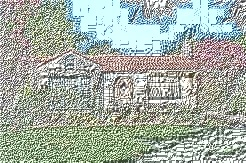
\includegraphics[width=0.45\textwidth]{./Figures/calhouse_236/56-resultado.jpg}
    }
%        \caption{Imagen Original. $\mathscr{H_Y}=0.207231$. $SSIM_R=1$. $SSIM_G=1$. $SSIM_B=1$}
\end{subfigure}
    ~ %add desired spacing between images. e. g. ~. \quad. \qquad. \hfill etc. 
      %(or a blank line to force the subfigure onto a new line)
      \begin{subfigure}[ID=1]{
      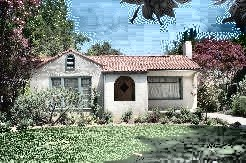
\includegraphics[width=0.45\textwidth]{./Figures/calhouse_236/61-resultado.jpg}   
      }
    %\begin{subfigure}[t]{0.45\textwidth}
%        \caption{Enhanced Image. $\mathscr{H_Y}=0.611275$. $SSIM_R=0.00897331$. $SSIM_G=0.00823064$. $SSIM_B=0.00851013$}
\end{subfigure}
    ~ %add desired spacing between images. e. g. ~. \quad. \qquad. \hfill etc. 
    %(or a blank line to force the subfigure onto a new line)
    \begin{subfigure}[ID=23]{
    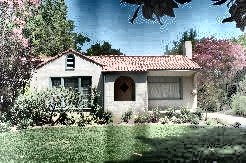
\includegraphics[width=0.45\textwidth]{./Figures/calhouse_236/82-resultado.jpg}
    }
    % \begin{subfigure}[t]{0.45\textwidth}
%        \caption{Enhanced Image.  $\mathscr{H_Y}=0.0350595$. $SSIM_R=0.416776$. $SSIM_G=0.403636$. $SSIM_B=0.417654$}
\end{subfigure} 
\begin{subfigure}[ID=24]{
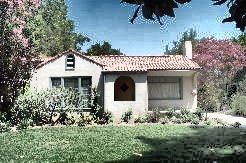
\includegraphics[width=0.45\textwidth]{./Figures/calhouse_236/101-resultado.jpg}
}
    % \begin{subfigure}[t]{0.45\textwidth}
        %\caption{Enhanced Image using \cite{morepso}. $\mathscr{H_Y}=0.788927$. $SSIM_R=0.000204143$. $SSIM_G=0.0000526475$. $SSIM_B=0.0000518143$}
        % \label{fig:calhouse23129}
        \end{subfigure}
    ~ %add desired spacing between images. e. g. ~. \quad. \qquad. \hfill etc. 
    %(or a blank line to force the subfigure onto a new line)
    \begin{subfigure}[ID=56]{
    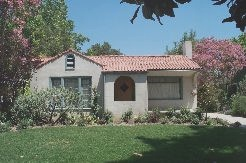
\includegraphics[width=0.45\textwidth]{./Figures/calhouse_236/107-resultado.jpg}
    }
    % \begin{subfigure}[t]{0.45\textwidth}
%        \caption{Enhanced Image.  $\mathscr{H_Y}=0.0350595$. $SSIM_R=0.416776$. $SSIM_G=0.403636$. $SSIM_B=0.417654$}
% \label{fig:calhouse231102}
\end{subfigure} 
\begin{subfigure}[Imagen Original]{
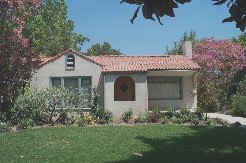
\includegraphics[width=0.45\textwidth]{./Figures/calhouse_236/calhouse_236.jpg}
}
    % \begin{subfigure}[t]{0.45\textwidth}
        %\caption{Enhanced Image using \cite{morepso}. $\mathscr{H_Y}=0.788927$. $SSIM_R=0.000204143$. $SSIM_G=0.0000526475$. $SSIM_B=0.0000518143$}
        % \label{fig:calhouse233orig}
        \end{subfigure}
        \caption{Imágenes visualmente relevantes obtenidas mediante $CMOPSO-CLAHE$. Las variables y decisión y métricas de las imágenes se muestran en la tabla \ref{tab:calhouse_234}.}
        \label{fig:anexocalhouse236}
        \end{figure}

        \begin{figure}[H]
        \centering
        %\begin{subfigure}[Gráfica de Frente Pareto para las soluciones no dominadas de \texttt{calhouse_231.jpg}]{
        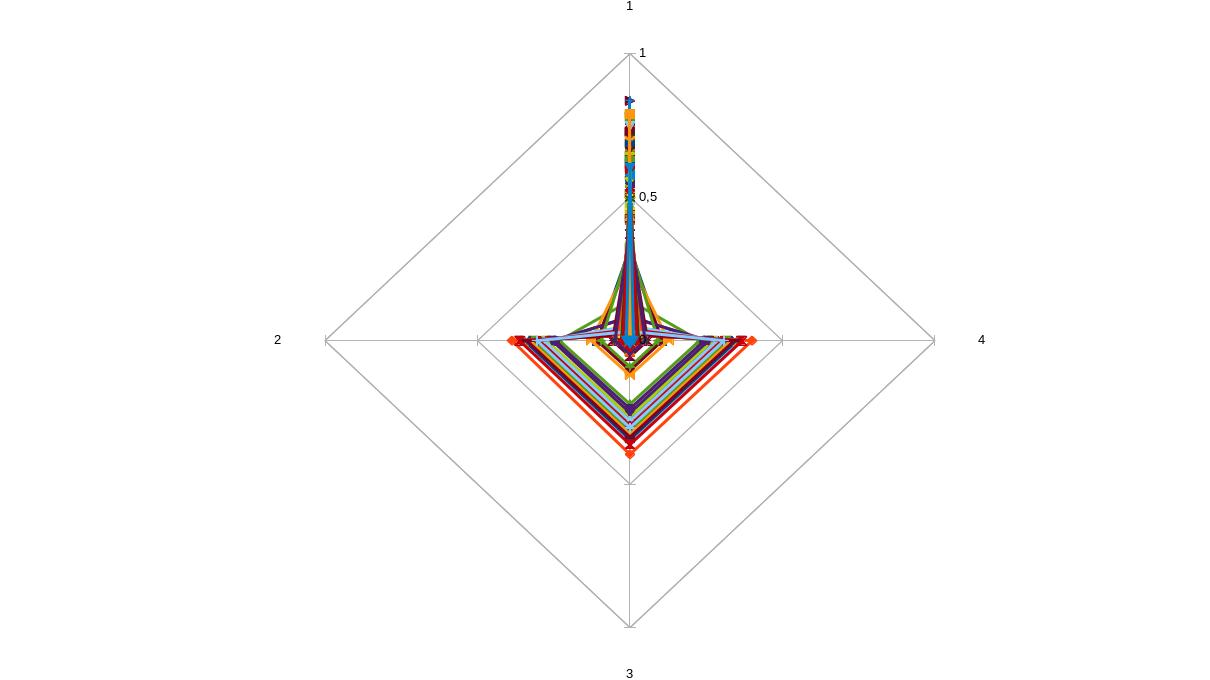
\includegraphics[width=\textwidth]{./Figures/calhouse_236/calhouse_236_2.jpg}
        %}
        %\end{subfigure}
        \caption{Frente pareto que contrasta los objetivos de las soluciones no dominadas. para los resultados de imágenes que se muestran en la tabla \ref{tab:calhouse_236}.}
        \label{fig:calhouse2362fp}
        \end{figure}



\section{Imagen de prueba \texttt{calhouse\_237.jpg}}

%calhouse 234
\scriptsize
\begin{longtable}{|c|c|c|c|c|c|c|c|}
% \centering
%\begin{tabular}
\hline
ID & $\mathscr{R}_x$ & $\mathscr{R}_y$ & $\mathscr{C}$ & $f_1(I.\vv{x})$ & $f_2(I.\vv{x})$ & $f_3(I.\vv{x})$ & $f_4(I.\vv{x})$ \\
\hline
0.0 & 3.05920559855 & 2.0 & 0.818377249473 & 0.527355 & 0.0266691 & 0.0245697 & 0.0257519 \\
1.0 & 59.4737222511 & 2.89333813993 & 0.348404050444 & 0.41236 & 0.10348 & 0.0946411 & 0.0973958 \\
2.0 & 2.0 & 2.0 & 0.839606904816 & 0.515146 & 0.029663 & 0.0272264 & 0.0286435 \\
3.0 & 12.9218206966 & 2.0 & 0.858950496855 & 0.524695 & 0.0260812 & 0.024745 & 0.0255167 \\
4.0 & 10.5861270573 & 2.0 & 1.0 & 0.494054 & 0.034029 & 0.032038 & 0.0331011 \\
5.0 & 2.0 & 2.0 & 0.738264702174 & 0.548753 & 0.0229975 & 0.0211807 & 0.0222653 \\
6.0 & 26.6275579915 & 5.94117149491 & 0.665067465025 & 0.445776 & 0.0921568 & 0.0871899 & 0.0896835 \\
7.0 & 40.2637323895 & 4.26908034048 & 0.515435272603 & 0.445821 & 0.0866204 & 0.0792098 & 0.0816776 \\
8.0 & 3.49067737033 & 2.93289641943 & 0.802799465668 & 0.511109 & 0.0287218 & 0.0274117 & 0.0284403 \\
9.0 & 3.22990336462 & 2.0 & 0.131123269978 & 0.793742 & 0.000731432 & 0.000664557 & 0.000679274 \\
10.0 & 10.3190985048 & 2.38672127726 & 0.707716171361 & 0.580588 & 0.0168114 & 0.0159317 & 0.0165228 \\
11.0 & 4.11320800645 & 2.168574578 & 0.819304542919 & 0.519737 & 0.027535 & 0.0255765 & 0.0267492 \\
12.0 & 2.0 & 2.0 & 0.0 & 0.138669 & 0.231124 & 0.221532 & 0.228493 \\
13.0 & 18.478878223 & 2.0 & 0.5 & 0.62303 & 0.00889421 & 0.00828233 & 0.00854233 \\
14.0 & 13.5120025697 & 2.0 & 0.973685974855 & 0.502234 & 0.0314391 & 0.0298899 & 0.0308901 \\
15.0 & 8.55347614302 & 2.3885548305 & 0.5 & 0.640419 & 0.00871692 & 0.00817691 & 0.00844283 \\
16.0 & 16.5523237023 & 2.08566454858 & 0.705975808503 & 0.574325 & 0.0167192 & 0.0159348 & 0.0164249 \\
17.0 & 7.94181429612 & 2.01898097636 & 0.376325532835 & 0.675727 & 0.00441494 & 0.00421142 & 0.00434589 \\
18.0 & 10.7801739126 & 2.03067519693 & 0.909204773465 & 0.513048 & 0.0288726 & 0.0272513 & 0.0282724 \\
19.0 & 11.7345388592 & 2.0 & 0.5 & 0.601996 & 0.0103419 & 0.00983332 & 0.010186 \\
20.0 & 7.46482984756 & 2.0 & 0.0 & 0.0413656 & 0.289774 & 0.282049 & 0.285934 \\
21.0 & 4.18534224416 & 2.15034089143 & 0.0881709349719 & 0.832464 & 0.000183395 & 0.000143403 & 0.000147903 \\
22.0 & 6.31141664605 & 2.0 & 0.67190050469 & 0.564373 & 0.0195332 & 0.0183163 & 0.019096 \\
23.0 & 3.24290009511 & 2.01332262327 & 0.419925814383 & 0.664902 & 0.00713225 & 0.00668782 & 0.00695413 \\
24.0 & 3.76729777581 & 2.00244613865 & 0.293584223893 & 0.730788 & 0.00268251 & 0.00253008 & 0.00260924 \\
25.0 & 2.0 & 2.0 & 0.727267809131 & 0.553606 & 0.021385 & 0.0196689 & 0.0206698 \\
26.0 & 5.41254148766 & 2.11295066377 & 0.200766112685 & 0.738358 & 0.00171736 & 0.0016441 & 0.00168794 \\
27.0 & 11.4788104348 & 2.0 & 0.35822182698 & 0.723333 & 0.00331185 & 0.00315496 & 0.00324682 \\
28.0 & 2.0 & 2.0 & 0.0155329642123 & 0.835548 & 0.000142314 & 0.000115598 & 0.000110237 \\
29.0 & 3.34190501004 & 2.0 & 0.306795075516 & 0.710093 & 0.00364066 & 0.0034385 & 0.00355669 \\
30.0 & 2.0 & 2.68568702251 & 0.893874350908 & 0.492458 & 0.0341363 & 0.0321934 & 0.0336531 \\
31.0 & 2.73364801795 & 2.03671285068 & 0.199177359771 & 0.755389 & 0.00142469 & 0.00136878 & 0.00139945 \\
32.0 & 5.97689620295 & 2.47617083604 & 0.769196682286 & 0.547824 & 0.0229913 & 0.0213657 & 0.0222196 \\
33.0 & 2.0 & 2.0 & 0.759973896268 & 0.54257 & 0.0246297 & 0.0226156 & 0.0237819 \\
34.0 & 2.0 & 2.0 & 0.91299851085 & 0.493326 & 0.0350073 & 0.032038 & 0.0337141 \\
35.0 & 5.69117526472 & 2.0 & 0.185206673924 & 0.78611 & 0.000841764 & 0.00080091 & 0.000816869 \\
36.0 & 3.31752390115 & 2.20034303022 & 0.0 & 0.0846047 & 0.245215 & 0.237309 & 0.244065 \\
37.0 & 14.8146022888 & 2.41520441876 & 0.5 & 0.666303 & 0.00554846 & 0.00524035 & 0.00540413 \\
38.0 & 5.35242082204 & 2.01490018104 & 0.445174122796 & 0.66294 & 0.00827245 & 0.00775234 & 0.00802141 \\
39.0 & 6.59894593875 & 2.0 & 0.236480112225 & 0.773407 & 0.00121588 & 0.00114323 & 0.00117378 \\
40.0 & 10.5583259467 & 2.0 & 0.0 & 0.0396638 & 0.306313 & 0.297956 & 0.302221 \\
41.0 & 3.79907581012 & 2.17255146371 & 0.805472933679 & 0.530471 & 0.0249754 & 0.0230687 & 0.0241613 \\
42.0 & 23.7942500622 & 2.0 & 0.950997765336 & 0.448877 & 0.0337654 & 0.0325268 & 0.0334449 \\
43.0 & 4.9173817596 & 2.0 & 0.0 & 0.0519104 & 0.273498 & 0.265907 & 0.270653 \\
44.0 & 2.57756770928 & 2.02337355103 & 0.720115798569 & 0.551425 & 0.0215359 & 0.0198995 & 0.0208231 \\
45.0 & 6.00125918588 & 2.43787950072 & 0.0 & 0.0493283 & 0.277246 & 0.269315 & 0.27368 \\
46.0 & 3.06766647761 & 2.6389908854 & 0.634646330157 & 0.571977 & 0.0180757 & 0.0172713 & 0.0179017 \\
47.0 & 14.3940487996 & 2.49699884946 & 0.524848751778 & 0.58597 & 0.01286 & 0.0122675 & 0.0126854 \\
48.0 & 2.73405360222 & 2.64939847282 & 0.685028650384 & 0.553035 & 0.0211689 & 0.0201818 & 0.0209119 \\
49.0 & 3.24897100584 & 2.0 & 0.463959307137 & 0.650707 & 0.00852852 & 0.00796836 & 0.00830184 \\
50.0 & 2.56237381612 & 2.06557090283 & 0.679025114903 & 0.557746 & 0.0203147 & 0.0187927 & 0.0196922 \\
51.0 & 23.4763470009 & 2.73175016325 & 0.0 & 0.0277634 & 0.406696 & 0.400567 & 0.40603 \\
52.0 & 7.43702560607 & 3.47215652036 & 0.0 & 0.0321503 & 0.363205 & 0.357271 & 0.362161 \\
53.0 & 18.8206167272 & 3.21670615569 & 0.0 & 0.0294476 & 0.401875 & 0.395903 & 0.401497 \\
54.0 & 3.46289153025 & 2.02262134397 & 0.0883240061534 & 0.829471 & 0.000258416 & 0.000220973 & 0.000231715 \\
55.0 & 2.0 & 3.42904893543 & 0.105680467779 & 0.831217 & 0.000254231 & 0.000202246 & 0.000220666 \\
56.0 & 10.9189634679 & 2.99856893327 & 0.0 & 0.0296307 & 0.381211 & 0.374829 & 0.380207 \\
57.0 & 6.21540270442 & 2.18648111809 & 0.899388322835 & 0.496642 & 0.0326795 & 0.0303633 & 0.0316357 \\
58.0 & 3.94192877805 & 2.0 & 0.864534440051 & 0.502655 & 0.0311266 & 0.0287067 & 0.03005 \\
59.0 & 2.0 & 2.71254442376 & 0.050929948535 & 0.836594 & 0.000146742 & 0.000117982 & 0.000110062 \\
60.0 & 18.3162941581 & 2.10331939107 & 0.804145499558 & 0.533793 & 0.0238637 & 0.022623 & 0.0232914 \\
61.0 & 19.6044912928 & 2.89298431286 & 0.0 & 0.0284328 & 0.402012 & 0.396043 & 0.401629 \\
62.0 & 2.0 & 2.0 & 0.0609928161487 & 0.787766 & 0.000256124 & 0.000197123 & 0.000228562 \\
63.0 & 3.8777168881 & 2.23805036326 & 0.52223536612 & 0.569097 & 0.0147406 & 0.0145173 & 0.0152212 \\
64.0 & 9.23675044508 & 2.35894152163 & 0.505589934566 & 0.576457 & 0.014684 & 0.0144162 & 0.015154 \\
65.0 & 15.0285552403 & 2.0 & 0.594417852291 & 0.523629 & 0.0229587 & 0.0225117 & 0.0233318 \\
66.0 & 3.29402722753 & 2.0 & 0.716236838749 & 0.483283 & 0.0287522 & 0.027986 & 0.0294905 \\
67.0 & 2.0 & 2.0 & 0.0 & 0.0819087 & 0.255368 & 0.251915 & 0.257656 \\
68.0 & 2.50152385245 & 2.0 & 0.269677482952 & 0.68885 & 0.00352479 & 0.00343585 & 0.00363311 \\
69.0 & 4.38930003576 & 2.0 & 0.177913813107 & 0.737098 & 0.0013308 & 0.00132604 & 0.00137942 \\
70.0 & 3.21131394196 & 2.20805639719 & 0.256319244386 & 0.699975 & 0.00309802 & 0.00307773 & 0.00326212 \\
71.0 & 2.0 & 2.0 & 0.572082014846 & 0.566152 & 0.0173144 & 0.0169155 & 0.0180509 \\
72.0 & 17.0343205121 & 2.0 & 0.501908060793 & 0.56284 & 0.0182472 & 0.017877 & 0.018825 \\
73.0 & 3.42849387459 & 2.0 & 0.470797316063 & 0.601152 & 0.0117493 & 0.0114363 & 0.0120534 \\
74.0 & 2.0 & 2.0 & 0.28762897403 & 0.684397 & 0.00417191 & 0.00409187 & 0.00435506 \\
75.0 & 2.0 & 2.0 & 0.319001035677 & 0.676598 & 0.00467596 & 0.00454571 & 0.00490102 \\
76.0 & 2.0 & 2.0 & 0.0467344262764 & 0.791656 & 0.000155317 & 0.000121572 & 0.000128309 \\
77.0 & 2.0 & 2.0 & 0.806851045046 & 0.449825 & 0.0362412 & 0.0352132 & 0.0377132 \\
78.0 & 2.53619847005 & 2.12229512798 & 0.706400893583 & 0.496626 & 0.0260506 & 0.02529 & 0.0266687 \\
79.0 & 2.0 & 2.0 & 0.22026142931 & 0.724546 & 0.00201504 & 0.00198291 & 0.00209202 \\
80.0 & 3.1496248741 & 2.35780181905 & 0.134385763543 & 0.748132 & 0.00104085 & 0.000998748 & 0.00106332 \\
81.0 & 2.0 & 2.0 & 0.264811557652 & 0.697151 & 0.00318869 & 0.00307715 & 0.00330749 \\
82.0 & 2.0 & 2.0 & 0.789976935473 & 0.461123 & 0.0335764 & 0.032814 & 0.0350383 \\
83.0 & 2.0 & 2.0 & 0.132666358022 & 0.758529 & 0.000769288 & 0.000722369 & 0.000767623 \\
84.0 & 3.0805059994 & 2.2464397548 & 0.996037935634 & 0.384975 & 0.0502797 & 0.0486287 & 0.051306 \\
85.0 & 2.42385569563 & 2.35114636574 & 0.192442273151 & 0.728299 & 0.00148275 & 0.00144158 & 0.00152957 \\
86.0 & 2.0 & 2.0 & 0.721958245867 & 0.494555 & 0.0270831 & 0.0264682 & 0.0282887 \\
87.0 & 3.88119197777 & 2.0 & 0.5 & 0.596839 & 0.0131762 & 0.0129074 & 0.0136321 \\
88.0 & 2.0 & 2.0 & 0.871233788733 & 0.431905 & 0.0403448 & 0.0392149 & 0.0419863 \\
89.0 & 2.0 & 2.23999622177 & 0.384270287837 & 0.648621 & 0.007755 & 0.00755259 & 0.00805606 \\
90.0 & 40.6606731155 & 3.89845113621 & 0.863744583938 & 0.297561 & 0.107656 & 0.103902 & 0.105838 \\
91.0 & 2.52539483027 & 2.435267208 & 0.0 & 0.0501919 & 0.282841 & 0.280242 & 0.285594 \\
92.0 & 4.27010672218 & 2.24683966603 & 0.229943686198 & 0.71229 & 0.00263194 & 0.00250156 & 0.00264687 \\
93.0 & 5.61645171759 & 2.0 & 0.55477863176 & 0.564425 & 0.0178416 & 0.0174361 & 0.0182652 \\
94.0 & 2.77372933045 & 2.18507455419 & 0.940781652341 & 0.389108 & 0.0487418 & 0.0471518 & 0.0496774 \\
95.0 & 53.0367396805 & 2.98530919662 & 0.274034660606 & 0.276232 & 0.127112 & 0.120837 & 0.125981 \\
96.0 & 14.6592957957 & 2.49920299096 & 0.0848652779147 & 0.684746 & 0.00401761 & 0.00395017 & 0.00417073 \\
97.0 & 2.56197289901 & 2.14221288416 & 0.903800468918 & 0.409682 & 0.0439377 & 0.0424819 & 0.044889 \\
98.0 & 2.27928718968 & 2.09259246829 & 0.948583037555 & 0.407068 & 0.0475321 & 0.0460638 & 0.0492886 \\
99.0 & 3.40767689992 & 2.0 & 0.0936325288752 & 0.777003 & 0.000383461 & 0.000322487 & 0.00035059 \\
100.0 & 2.00071972546 & 2.18715878718 & 0.0822339049711 & 0.775215 & 0.000484727 & 0.000458843 & 0.000490921 \\
101.0 & 3.18849968748 & 2.11721552178 & 0.669535264594 & 0.516613 & 0.0230328 & 0.0225424 & 0.0237412 \\
102.0 & 2.93693151672 & 2.0 & 0.000663482307116 & 0.780215 & 0.0003251 & 0.000293507 & 0.000313995 \\
103.0 & 8.65231777983 & 2.25641057173 & 0.309579061915 & 0.671622 & 0.00477057 & 0.00471242 & 0.00498622 \\
104.0 & 4.17465507278 & 2.0 & 0.905279192884 & 0.420893 & 0.0414817 & 0.0404199 & 0.0424878 \\
105.0 & 3.19164752264 & 2.15674021667 & 0.78506628645 & 0.46783 & 0.0316 & 0.0307277 & 0.0323041 \\
106.0 & 4.94550285783 & 2.0 & 0.579659528424 & 0.542229 & 0.0191408 & 0.0188228 & 0.0197266 \\
107.0 & 5.38258312293 & 2.18174297069 & 0.696056694267 & 0.494868 & 0.0275482 & 0.0270448 & 0.0282753 \\
108.0 & 2.60045407436 & 2.05878290217 & 0.833889686802 & 0.434412 & 0.0382984 & 0.0371935 & 0.0391734 \\
109.0 & 2.89274081964 & 2.09244388982 & 0.5 & 0.578231 & 0.0139116 & 0.0136808 & 0.0144633 \\
110.0 & 4.46612236884 & 2.00400822418 & 0.41014792752 & 0.615799 & 0.0091199 & 0.00902098 & 0.00947175 \\
111.0 & 2.32027716334 & 2.19828799908 & 0.116924112842 & 0.767094 & 0.000488963 & 0.000461673 & 0.000486079 \\
112.0 & 5.83793108238 & 2.0 & 0.715864343637 & 0.493677 & 0.0276822 & 0.0271113 & 0.0282399 \\
113.0 & 3.06989158301 & 2.16188589823 & 0.883057280032 & 0.423313 & 0.0410583 & 0.0397921 & 0.0418922 \\
114.0 & 11.046678087 & 3.23289644879 & 0.496094870334 & 0.59462 & 0.0135325 & 0.0132879 & 0.0138825 \\
115.0 & 22.2867943733 & 6.76007972721 & 0.605211850181 & 0.322022 & 0.106831 & 0.102759 & 0.104597 \\
116.0 & 6.0946668293 & 2.0 & 0.662951872774 & 0.528742 & 0.0214838 & 0.0210648 & 0.0219197 \\
117.0 & 3.08232250949 & 2.20243292212 & 0.589903990702 & 0.547642 & 0.018305 & 0.0179109 & 0.0189608 \\
118.0 & 14.1272541585 & 2.0 & 0.0 & 0.0210977 & 0.346013 & 0.344528 & 0.350455 \\
119.0 & 2.0 & 32.1008881344 & 0.0 & 0.0200801 & 0.386856 & 0.396321 & 0.400445 \\
120.0 & 2.57045354819 & 2.29835583567 & 0.360097508676 & 0.656688 & 0.00595517 & 0.00589545 & 0.00621782 \\
121.0 & 18.3908408564 & 2.00907262538 & 0.220320957492 & 0.677333 & 0.00469509 & 0.00463112 & 0.00484218 \\
122.0 & 5.09101232485 & 2.08208724433 & 0.789057270207 & 0.459602 & 0.0343625 & 0.0337502 & 0.0353585 \\
123.0 & 4.33875233106 & 2.37394019484 & 0.626022843896 & 0.524631 & 0.0212356 & 0.0208217 & 0.0219233 \\
124.0 & 2.89910129784 & 2.09857012232 & 0.620619466995 & 0.531118 & 0.0207645 & 0.0202031 & 0.0212407 \\
125.0 & 6.69112541772 & 2.0 & 0.0808171853509 & 0.753023 & 0.000811243 & 0.000784616 & 0.000827166 \\
126.0 & 4.02357529673 & 2.28180974255 & 0.723377786697 & 0.486755 & 0.0280603 & 0.0274114 & 0.0289443 \\
127.0 & 4.97130982878 & 2.0 & 1.0 & 0.371791 & 0.056858 & 0.05543 & 0.0578333 \\
128.0 & 4.53365585341 & 2.28374929046 & 0.660447936924 & 0.511524 & 0.0248132 & 0.0243987 & 0.0254811 \\
129.0 & 9.84533116319 & 2.0 & 0.0 & 0.023551 & 0.3383 & 0.336246 & 0.342151 \\
130.0 & 3.97161734121 & 2.25443091293 & 0.76048571887 & 0.462856 & 0.033901 & 0.033062 & 0.0347065 \\
131.0 & 6.78695520669 & 2.12521973727 & 0.351567803707 & 0.651144 & 0.00780234 & 0.00755867 & 0.00787006 \\
132.0 & 9.9272458829 & 2.0 & 0.272256715287 & 0.660394 & 0.00547086 & 0.00543164 & 0.00569884 \\
133.0 & 4.33916600812 & 2.25997246393 & 0.661379412447 & 0.507441 & 0.0256752 & 0.0251247 & 0.0263251 \\
134.0 & 3.19954671808 & 2.00008364564 & 0.208077021581 & 0.726163 & 0.00205421 & 0.00196918 & 0.00206596 \\
135.0 & 3.66180288093 & 2.00785877492 & 0.281242886046 & 0.681593 & 0.00418639 & 0.00415261 & 0.00438053 \\
136.0 & 4.01477248204 & 2.0 & 0.0 & 0.0386662 & 0.298298 & 0.2962 & 0.301126 \\
137.0 & 5.13577954402 & 2.0 & 0.0 & 0.0321527 & 0.30536 & 0.30339 & 0.308505 \\
138.0 & 6.18550525031 & 2.07582545219 & 0.454041235272 & 0.598613 & 0.0118493 & 0.0117448 & 0.0121879 \\
139.0 & 11.7907719695 & 4.45920706214 & 0.320240239639 & 0.602102 & 0.0113926 & 0.0111123 & 0.0113819 \\
140.0 & 2.57117669398 & 2.0 & 0.80371799535 & 0.451618 & 0.0344522 & 0.0333763 & 0.0352578 \\
141.0 & 3.4459959327 & 2.26819149355 & 0.383498913972 & 0.631119 & 0.00848167 & 0.00827093 & 0.00872122 \\
142.0 & 5.7743704931 & 2.02600626626 & 0.0 & 0.0297699 & 0.316537 & 0.313988 & 0.319524 \\
143.0 & 8.11722209141 & 2.0 & 0.0 & 0.0249429 & 0.328823 & 0.326689 & 0.332172 \\
144.0 & 3.24600231042 & 2.0266912741 & 0.181037050653 & 0.740656 & 0.0012681 & 0.00124621 & 0.00131296 \\
145.0 & 10.6575098171 & 2.06493027536 & 0.0 & 0.0218916 & 0.338454 & 0.336511 & 0.342515 \\
146.0 & 2.04879138969 & 2.92668548199 & 0.37128123925 & 0.654835 & 0.00737856 & 0.00732287 & 0.00799174 \\
147.0 & 39.3147845245 & 2.0 & 0.0 & 0.0200915 & 0.362392 & 0.36188 & 0.368223 \\
148.0 & 3.98674405538 & 2.3160088163 & 0.303661922608 & 0.66859 & 0.00505159 & 0.0049349 & 0.00521387 \\
149.0 & 12.1956325322 & 2.05767989569 & 0.0 & 0.0213795 & 0.343065 & 0.341144 & 0.347002 \\
150.0 & 9.58370911975 & 2.0 & 0.5 & 0.550348 & 0.0184473 & 0.018058 & 0.0188672 \\
151.0 & 6.95607599159 & 2.39985184776 & 0.548214261218 & 0.568738 & 0.0171921 & 0.0167467 & 0.0174151 \\
152.0 & 13.1046475652 & 2.16550356932 & 0.339020894713 & 0.638225 & 0.00777391 & 0.0076255 & 0.00791422 \\
153.0 & 6.92405987133 & 2.0 & 0.5 & 0.596471 & 0.0133184 & 0.013128 & 0.0137713 \\
154.0 & 2.0 & 3.47365110684 & 0.0228472647706 & 0.789495 & 0.00022413 & 0.0001983 & 0.000207669 \\
155.0 & 29.1681595253 & 5.16137124197 & 0.803710536145 & 0.330317 & 0.0943822 & 0.0913762 & 0.0924006 \\
156.0 & 3.91219588449 & 2.0 & 0.287960717289 & 0.730788 & 0.00268251 & 0.00253008 & 0.00260924 \\
157.0 & 2.0 & 2.0 & 0.0453845246446 & 0.835548 & 0.000142314 & 0.000115598 & 0.000110237 \\
158.0 & 7.10968787997 & 2.16243789429 & 0.0 & 0.0413656 & 0.289774 & 0.282049 & 0.285934 \\
159.0 & 2.0 & 2.0 & 0.0 & 0.138669 & 0.231124 & 0.221532 & 0.228493 \\
160.0 & 60.2601330234 & 3.14765020916 & 0.00140994587414 & 0.41236 & 0.10348 & 0.0946411 & 0.0973958 \\
161.0 & 6.86383645084 & 3.22650755844 & 0.0 & 0.0321503 & 0.363205 & 0.357271 & 0.362161 \\
162.0 & 4.92519696161 & 2.0 & 0.0 & 0.0519104 & 0.273498 & 0.265907 & 0.270653 \\
163.0 & 6.86383645084 & 2.0 & 0.206906460129 & 0.773407 & 0.00121588 & 0.00114323 & 0.00117378 \\
164.0 & 3.01646754415 & 2.03540078442 & 0.322271985499 & 0.710093 & 0.00364066 & 0.0034385 & 0.00355669 \\
165.0 & 2.0 & 2.69749980273 & 0.029768001776 & 0.836594 & 0.000146742 & 0.000117982 & 0.000110062 \\
166.0 & 3.19042336647 & 2.18844893672 & 0.0 & 0.0846047 & 0.245215 & 0.237309 & 0.244065 \\
167.0 & 14.8781356558 & 2.0 & 0.547945552478 & 0.666303 & 0.00554846 & 0.00524035 & 0.00540413 \\
168.0 & 3.00091756809 & 2.0 & 0.0853731927042 & 0.829471 & 0.000258416 & 0.000220973 & 0.000231715 \\
169.0 & 2.07261258297 & 2.00925484302 & 0.72869127062 & 0.553606 & 0.021385 & 0.0196689 & 0.0206698 \\
170.0 & 3.02449918773 & 2.0 & 0.136800145681 & 0.793742 & 0.000731432 & 0.000664557 & 0.000679274 \\
171.0 & 3.93036926039 & 2.10024471763 & 0.0163575505064 & 0.832464 & 0.000183395 & 0.000143403 & 0.000147903 \\
172.0 & 2.93495296342 & 2.00011405046 & 0.217635951343 & 0.755389 & 0.00142469 & 0.00136878 & 0.00139945 \\
173.0 & 18.445487497 & 2.00156786658 & 0.636800145681 & 0.62303 & 0.00889421 & 0.00828233 & 0.00854233 \\
174.0 & 2.0 & 2.0 & 0.769040550106 & 0.54257 & 0.0246297 & 0.0226156 & 0.0237819 \\
175.0 & 7.87557599448 & 2.01980665798 & 0.323462111002 & 0.675727 & 0.00441494 & 0.00421142 & 0.00434589 \\
176.0 & 2.71384977033 & 2.03677751715 & 0.685598343219 & 0.557746 & 0.0203147 & 0.0187927 & 0.0196922 \\
177.0 & 17.1606165667 & 2.04973266997 & 0.645496357561 & 0.574325 & 0.0167192 & 0.0159348 & 0.0164249 \\
178.0 & 6.07070665459 & 2.0 & 0.0 & 0.0493283 & 0.277246 & 0.269315 & 0.27368 \\
179.0 & 3.1517051808 & 2.04393353452 & 0.459463481702 & 0.650707 & 0.00852852 & 0.00796836 & 0.00830184 \\
180.0 & 10.6495599986 & 2.0 & 0.0 & 0.0396638 & 0.306313 & 0.297956 & 0.302221 \\
181.0 & 20.1008460783 & 3.40092314672 & 0.0 & 0.0284328 & 0.402012 & 0.396043 & 0.401629 \\
182.0 & 35.8664681277 & 3.60814885455 & 0.277432850843 & 0.445821 & 0.0866204 & 0.0792098 & 0.0816776 \\
183.0 & 2.0 & 2.0 & 0.747676874116 & 0.548753 & 0.0229975 & 0.0211807 & 0.0222653 \\
184.0 & 14.141309048 & 2.03663320568 & 1.0 & 0.502234 & 0.0314391 & 0.0298899 & 0.0308901 \\
185.0 & 12.4361275039 & 2.0 & 0.5 & 0.601996 & 0.0103419 & 0.00983332 & 0.010186 \\
186.0 & 10.8935616455 & 3.11138787505 & 0.0 & 0.0296307 & 0.381211 & 0.374829 & 0.380207 \\
187.0 & 11.1967964551 & 2.0 & 0.377393429315 & 0.723333 & 0.00331185 & 0.00315496 & 0.00324682 \\
188.0 & 2.0 & 2.76240797431 & 0.893352619616 & 0.492458 & 0.0341363 & 0.0321934 & 0.0336531 \\
189.0 & 10.3888630345 & 2.48373038733 & 0.644314916717 & 0.580588 & 0.0168114 & 0.0159317 & 0.0165228 \\
190.0 & 23.5939286353 & 2.06576849445 & 1.0 & 0.448877 & 0.0337654 & 0.0325268 & 0.0334449 \\
191.0 & 13.5110705465 & 2.0 & 0.537105312897 & 0.58597 & 0.01286 & 0.0122675 & 0.0126854 \\
192.0 & 11.161174392 & 2.0 & 1.0 & 0.494054 & 0.034029 & 0.032038 & 0.0331011 \\
193.0 & 2.01955008243 & 2.01429153788 & 0.835398992861 & 0.515146 & 0.029663 & 0.0272264 & 0.0286435 \\
194.0 & 4.32373349191 & 2.0 & 0.898296732518 & 0.502655 & 0.0311266 & 0.0287067 & 0.03005 \\
195.0 & 18.0312224513 & 2.04695536264 & 0.793770605476 & 0.533793 & 0.0238637 & 0.022623 & 0.0232914 \\
196.0 & 9.27907147183 & 2.0 & 0.514620698238 & 0.640419 & 0.00871692 & 0.00817691 & 0.00844283 \\
197.0 & 3.23445968917 & 2.04213840034 & 0.723171113862 & 0.551425 & 0.0215359 & 0.0198995 & 0.0208231 \\
198.0 & 5.70191481922 & 2.0 & 0.671980206361 & 0.564373 & 0.0195332 & 0.0183163 & 0.019096 \\
199.0 & 3.8031006825 & 2.10206303901 & 0.816463208942 & 0.519737 & 0.027535 & 0.0255765 & 0.0267492 \\
200.0 & 2.0 & 2.00309672919 & 0.929927397784 & 0.493326 & 0.0350073 & 0.032038 & 0.0337141 \\
201.0 & 23.0934440833 & 2.87820318114 & 0.0 & 0.0277634 & 0.406696 & 0.400567 & 0.40603 \\
202.0 & 12.8873870019 & 3.34712555457 & 0.0 & 0.0292034 & 0.390222 & 0.383769 & 0.389344 \\
203.0 & 4.99834352306 & 2.0 & 0.231161071546 & 0.738358 & 0.00171736 & 0.0016441 & 0.00168794 \\
204.0 & 3.93542864255 & 2.00482607601 & 0.76242369505 & 0.530471 & 0.0249754 & 0.0230687 & 0.0241613 \\
205.0 & 5.81434568466 & 2.0 & 0.83094817677 & 0.518807 & 0.027765 & 0.0259249 & 0.0270216 \\
206.0 & 3.43255891831 & 2.75334997089 & 0.78520955672 & 0.511109 & 0.0287218 & 0.0274117 & 0.0284403 \\
207.0 & 5.9810515342 & 2.04126607724 & 0.217700391634 & 0.78611 & 0.000841764 & 0.00080091 & 0.000816869 \\
208.0 & 4.5854733528 & 2.5699510791 & 0.894571204573 & 0.507807 & 0.0309136 & 0.0296258 & 0.0305795 \\
209.0 & 3.42411147492 & 2.70269682241 & 0.7238271912 & 0.553035 & 0.0211689 & 0.0201818 & 0.0209119 \\
210.0 & 12.8025518818 & 2.10496122072 & 0.965321243034 & 0.524695 & 0.0260812 & 0.024745 & 0.0255167 \\
211.0 & 4.15856964429 & 3.33319055364 & 0.419356255648 & 0.65922 & 0.00689137 & 0.00665012 & 0.00686885 \\
212.0 & 5.64296207359 & 2.27505388298 & 0.909955923922 & 0.496642 & 0.0326795 & 0.0303633 & 0.0316357 \\
213.0 & 2.90425617605 & 2.00261820264 & 0.810192803646 & 0.527355 & 0.0266691 & 0.0245697 & 0.0257519 \\
214.0 & 2.0 & 2.55724680535 & 0.112366689345 & 0.831217 & 0.000254231 & 0.000202246 & 0.000220666 \\
215.0 & 2.52005852154 & 2.54096940413 & 0.57469112061 & 0.582351 & 0.0151525 & 0.0144716 & 0.0149766 \\
217.0 & 2.0 & 2.0 & 0.0 & 0.0836768 & 0.307048 & 0.302543 & 0.327743 \\
218.0 & 59.8648822215 & 3.10648952891 & 0.444966434956 & 0.478651 & 0.119989 & 0.11423 & 0.119011 \\
219.0 & 2.59508826964 & 2.0 & 0.0 & 0.0556154 & 0.308506 & 0.30849 & 0.330852 \\
224.0 & 3.66225847821 & 2.21580184686 & 0.0757012666101 & 0.951972 & 0.000126514 & 8.90623e-05 & 0.000108992 \\
228.0 & 3.48651871661 & 2.07314587592 & 0.105336898278 & 0.941825 & 0.000189923 & 0.000162224 & 0.000181752 \\
232.0 & 5.32157449666 & 2.0 & 0.0 & 0.0305114 & 0.317932 & 0.322037 & 0.341985 \\
234.0 & 2.65001691077 & 2.02156004558 & 0.120047605247 & 0.919156 & 0.000603614 & 0.00058067 & 0.000637189 \\
236.0 & 13.1810409121 & 3.23517870856 & 0.0 & 0.0131516 & 0.380016 & 0.392326 & 0.41105 \\
238.0 & 9.72023471302 & 2.0 & 0.0 & 0.0208297 & 0.331318 & 0.33796 & 0.35694 \\
239.0 & 2.0 & 3.28751087299 & 0.0461235500575 & 0.952027 & 0.000116321 & 8.60916e-05 & 9.15212e-05 \\
240.0 & 2.00000757002 & 2.0 & 0.130742260328 & 0.927542 & 0.000485918 & 0.000482601 & 0.000502934 \\
241.0 & 3.658809558 & 2.46749747997 & 0.0 & 0.0340362 & 0.315724 & 0.319053 & 0.339249 \\
245.0 & 6.14970752169 & 2.0 & 0.0 & 0.0238304 & 0.323505 & 0.327812 & 0.34729 \\
247.0 & 3.46583677145 & 2.18538621265 & 0.0323987519322 & 0.950603 & 0.000190459 & 0.0001664 & 0.000169953 \\
249.0 & 15.4346519823 & 2.85934393756 & 0.0 & 0.0125618 & 0.380785 & 0.392875 & 0.411493 \\
254.0 & 7.07601509571 & 2.86706706754 & 0.0 & 0.0181489 & 0.365409 & 0.37581 & 0.395036 \\
256.0 & 36.7565571504 & 3.95351146599 & 1.0 & 0.544655 & 0.101971 & 0.0980491 & 0.101015 \\
262.0 & 17.6117632209 & 2.0 & 0.0 & 0.0192766 & 0.340929 & 0.34925 & 0.367757 \\
269.0 & 21.9684100936 & 2.48648213616 & 0.0 & 0.018476 & 0.342172 & 0.350797 & 0.36937 \\
272.0 & 7.91366262721 & 2.98767140446 & 0.0 & 0.0155859 & 0.367961 & 0.378913 & 0.397759 \\
273.0 & 18.8997331385 & 2.55535529363 & 0.0 & 0.012115 & 0.386146 & 0.398668 & 0.4169 \\
274.0 & 10.7766620737 & 2.58811481362 & 0.0 & 0.0131903 & 0.375809 & 0.387382 & 0.405952 \\
275.0 & 15.0012576384 & 2.0 & 0.0 & 0.0202694 & 0.337863 & 0.345654 & 0.364441 \\
280.0 & 23.3412573476 & 3.45068257592 & 0.0 & 0.0120707 & 0.388381 & 0.400829 & 0.419208 \\
281.0 & 2.0 & 29.2537611897 & 0.0 & 0.0200801 & 0.386856 & 0.396321 & 0.400445 \\
282.0 & 22.1696868766 & 6.95311768547 & 0.318328909142 & 0.322022 & 0.106831 & 0.102759 & 0.104597 \\
283.0 & 11.7588192424 & 4.06004938476 & 0.383857283857 & 0.602102 & 0.0113926 & 0.0111123 & 0.0113819 \\
284.0 & 2.0 & 2.0 & 0.0319478654931 & 0.791656 & 0.000155317 & 0.000121572 & 0.000128309 \\
285.0 & 28.3238841117 & 2.0 & 0.0 & 0.0209365 & 0.359519 & 0.358839 & 0.365177 \\
286.0 & 2.0 & 2.0 & 0.880475877077 & 0.431905 & 0.0403448 & 0.0392149 & 0.0419863 \\
287.0 & 2.98467735884 & 2.0 & 0.46973075042 & 0.601152 & 0.0117493 & 0.0114363 & 0.0120534 \\
288.0 & 2.0 & 2.0 & 0.0 & 0.0819087 & 0.255368 & 0.251915 & 0.257656 \\
289.0 & 41.2967508657 & 2.0 & 0.0 & 0.0200915 & 0.362392 & 0.36188 & 0.368223 \\
290.0 & 4.41001381809 & 2.0 & 0.642831911216 & 0.524631 & 0.0212356 & 0.0208217 & 0.0219233 \\
291.0 & 2.0 & 2.0 & 0.126434332289 & 0.758529 & 0.000769288 & 0.000722369 & 0.000767623 \\
292.0 & 2.00236071465 & 2.0 & 0.187165015534 & 0.728299 & 0.00148275 & 0.00144158 & 0.00152957 \\
293.0 & 2.64119407356 & 2.0 & 1.0 & 0.384975 & 0.0502797 & 0.0486287 & 0.051306 \\
294.0 & 2.0 & 2.0 & 0.21438478586 & 0.724546 & 0.00201504 & 0.00198291 & 0.00209202 \\
295.0 & 17.6327136483 & 2.0 & 0.44003863696 & 0.677333 & 0.00469509 & 0.00463112 & 0.00484218 \\
296.0 & 2.0 & 2.0 & 0.815769788685 & 0.449825 & 0.0362412 & 0.0352132 & 0.0377132 \\
297.0 & 3.05635839198 & 2.0 & 0.00186259685548 & 0.780215 & 0.0003251 & 0.000293507 & 0.000313995 \\
298.0 & 5.34672838506 & 2.0 & 1.0 & 0.371791 & 0.056858 & 0.05543 & 0.0578333 \\
299.0 & 3.42674959155 & 2.34179763383 & 0.5 & 0.578231 & 0.0139116 & 0.0136808 & 0.0144633 \\
300.0 & 6.97469363828 & 2.02041799319 & 0.355159111635 & 0.651144 & 0.00780234 & 0.00755867 & 0.00787006 \\
301.0 & 2.0 & 2.0 & 0.796726639699 & 0.461123 & 0.0335764 & 0.032814 & 0.0350383 \\
302.0 & 9.87760847344 & 2.00351223834 & 0.551587997287 & 0.550348 & 0.0184473 & 0.018058 & 0.0188672 \\
303.0 & 3.14215228842 & 2.09534017996 & 0.39807189464 & 0.631119 & 0.00848167 & 0.00827093 & 0.00872122 \\
304.0 & 40.9282284971 & 3.89654873766 & 0.511910001518 & 0.297561 & 0.107656 & 0.103902 & 0.105838 \\
305.0 & 4.68568036259 & 2.0 & 0.811583976836 & 0.459602 & 0.0343625 & 0.0337502 & 0.0353585 \\
306.0 & 28.5089478284 & 4.95091993541 & 0.472570449467 & 0.330317 & 0.0943822 & 0.0913762 & 0.0924006 \\
307.0 & 51.9338366004 & 3.38024300284 & 0.467553715357 & 0.276232 & 0.127112 & 0.120837 & 0.125981 \\
308.0 & 2.91571180394 & 2.0 & 0.295440402212 & 0.68885 & 0.00352479 & 0.00343585 & 0.00363311 \\
309.0 & 2.0 & 2.5284076504 & 0.00233247253705 & 0.789495 & 0.00022413 & 0.0001983 & 0.000207669 \\
310.0 & 13.849631977 & 2.0 & 0.0 & 0.0210977 & 0.346013 & 0.344528 & 0.350455 \\
311.0 & 7.36572243027 & 2.33133713962 & 0.022347027078 & 0.753023 & 0.000811243 & 0.000784616 & 0.000827166 \\
312.0 & 2.54264486892 & 2.23187035974 & 0.927104611181 & 0.409682 & 0.0439377 & 0.0424819 & 0.044889 \\
313.0 & 2.0 & 2.0 & 0.322879861517 & 0.676598 & 0.00467596 & 0.00454571 & 0.00490102 \\
314.0 & 9.38695881887 & 2.02548326201 & 0.5 & 0.576457 & 0.014684 & 0.0144162 & 0.015154 \\
315.0 & 8.85336831037 & 2.0 & 0.225846688107 & 0.671622 & 0.00477057 & 0.00471242 & 0.00498622 \\
316.0 & 6.77924348173 & 2.03596655749 & 0.5 & 0.596471 & 0.0133184 & 0.013128 & 0.0137713 \\
317.0 & 10.5657715894 & 3.20721107006 & 0.498546660001 & 0.59462 & 0.0135325 & 0.0132879 & 0.0138825 \\
318.0 & 6.28685976041 & 2.01052710112 & 0.647832913503 & 0.528742 & 0.0214838 & 0.0210648 & 0.0219197 \\
319.0 & 2.0 & 2.0 & 0.283780299797 & 0.684397 & 0.00417191 & 0.00409187 & 0.00435506 \\
320.0 & 2.28894123207 & 2.0 & 0.950159554231 & 0.407068 & 0.0475321 & 0.0460638 & 0.0492886 \\
321.0 & 2.0 & 2.0138469561 & 0.574515501436 & 0.566152 & 0.0173144 & 0.0169155 & 0.0180509 \\
322.0 & 11.3130071317 & 2.0 & 0.0 & 0.0218916 & 0.338454 & 0.336511 & 0.342515 \\
323.0 & 5.02070659473 & 2.0 & 0.565238723806 & 0.542229 & 0.0191408 & 0.0188228 & 0.0197266 \\
324.0 & 2.51394293081 & 2.0010981024 & 0.225443613753 & 0.726163 & 0.00205421 & 0.00196918 & 0.00206596 \\
325.0 & 7.01754628434 & 2.4331168379 & 0.563825381965 & 0.568738 & 0.0171921 & 0.0167467 & 0.0174151 \\
326.0 & 4.10898278778 & 2.0 & 0.689747601695 & 0.507441 & 0.0256752 & 0.0251247 & 0.0263251 \\
327.0 & 3.7145161348 & 2.09457089838 & 0.171961414151 & 0.737098 & 0.0013308 & 0.00132604 & 0.00137942 \\
328.0 & 15.136276192 & 2.0 & 0.021216763623 & 0.684746 & 0.00401761 & 0.00395017 & 0.00417073 \\
329.0 & 3.55334595833 & 2.30312000801 & 0.28747541953 & 0.681593 & 0.00418639 & 0.00415261 & 0.00438053 \\
330.0 & 2.0 & 2.0 & 0.728372921272 & 0.494555 & 0.0270831 & 0.0264682 & 0.0282887 \\
331.0 & 2.63333144595 & 2.0 & 0.651497604432 & 0.516613 & 0.0230328 & 0.0225424 & 0.0237412 \\
332.0 & 3.20050272647 & 2.48503775324 & 0.634696158772 & 0.531118 & 0.0207645 & 0.0202031 & 0.0212407 \\
333.0 & 2.77289604321 & 2.0 & 0.778562248594 & 0.46783 & 0.0316 & 0.0307277 & 0.0323041 \\
334.0 & 3.68177436532 & 2.2002570085 & 0.709744325383 & 0.486755 & 0.0280603 & 0.0274114 & 0.0289443 \\
335.0 & 3.83528067928 & 2.0 & 0.5 & 0.596839 & 0.0131762 & 0.0129074 & 0.0136321 \\
336.0 & 8.04518063121 & 2.21037668395 & 0.0 & 0.0249429 & 0.328823 & 0.326689 & 0.332172 \\
337.0 & 3.53633170386 & 2.18668030624 & 0.0 & 0.0386662 & 0.298298 & 0.2962 & 0.301126 \\
338.0 & 2.0 & 2.0 & 0.270803360372 & 0.697151 & 0.00318869 & 0.00307715 & 0.00330749 \\
339.0 & 4.57568751792 & 2.0 & 0.742033669416 & 0.494868 & 0.0275482 & 0.0270448 & 0.0282753 \\
340.0 & 3.38804234892 & 2.02494407227 & 0.973287369237 & 0.389108 & 0.0487418 & 0.0471518 & 0.0496774 \\
341.0 & 3.18897880048 & 2.02453624939 & 0.369967092264 & 0.656688 & 0.00595517 & 0.00589545 & 0.00621782 \\
342.0 & 2.0 & 2.03517683157 & 0.10904947637 & 0.767094 & 0.000488963 & 0.000461673 & 0.000486079 \\
343.0 & 3.81380043203 & 2.0 & 0.764033263745 & 0.462856 & 0.033901 & 0.033062 & 0.0347065 \\
344.0 & 2.84152736761 & 2.27184182482 & 0.227222706704 & 0.699975 & 0.00309802 & 0.00307773 & 0.00326212 \\
345.0 & 2.0 & 2.0 & 0.0561204388478 & 0.787766 & 0.000256124 & 0.000197123 & 0.000228562 \\
346.0 & 6.14260698673 & 2.05804575351 & 0.484357127464 & 0.598613 & 0.0118493 & 0.0117448 & 0.0121879 \\
347.0 & 4.80462012006 & 2.0 & 0.653748848921 & 0.511524 & 0.0248132 & 0.0243987 & 0.0254811 \\
348.0 & 10.3524824338 & 2.08173317549 & 0.0 & 0.023551 & 0.3383 & 0.336246 & 0.342151 \\
349.0 & 3.09490078148 & 2.0 & 0.86673031869 & 0.423313 & 0.0410583 & 0.0397921 & 0.0418922 \\
350.0 & 3.42274397501 & 2.0 & 0.68370615374 & 0.496626 & 0.0260506 & 0.02529 & 0.0266687 \\
351.0 & 6.00196093315 & 2.0 & 0.711375545939 & 0.493677 & 0.0276822 & 0.0271113 & 0.0282399 \\
352.0 & 6.20968355369 & 2.06485703078 & 0.522945184834 & 0.564425 & 0.0178416 & 0.0174361 & 0.0182652 \\
353.0 & 3.33354268828 & 2.49739710414 & 0.127657729971 & 0.748132 & 0.00104085 & 0.000998748 & 0.00106332 \\
354.0 & 4.44451080114 & 2.25652976618 & 0.412301053221 & 0.615799 & 0.0091199 & 0.00902098 & 0.00947175 \\
355.0 & 2.0 & 2.0 & 0.0913383058808 & 0.775215 & 0.000484727 & 0.000458843 & 0.000490921 \\
356.0 & 4.78690119462 & 2.08742071362 & 0.0 & 0.0321527 & 0.30536 & 0.30339 & 0.308505 \\
357.0 & 4.4528374924 & 2.00440263579 & 0.857299954436 & 0.420893 & 0.0414817 & 0.0404199 & 0.0424878 \\
358.0 & 12.8225330218 & 2.0224902465 & 0.422948832258 & 0.638225 & 0.00777391 & 0.0076255 & 0.00791422 \\
359.0 & 2.0 & 2.70670840858 & 0.347976815513 & 0.654835 & 0.00737856 & 0.00732287 & 0.00799174 \\
360.0 & 2.78430052804 & 2.0 & 0.0 & 0.0501919 & 0.282841 & 0.280242 & 0.285594 \\
361.0 & 3.59413031562 & 2.08927500131 & 0.344871035313 & 0.66859 & 0.00505159 & 0.0049349 & 0.00521387 \\
362.0 & 2.78091678085 & 2.00872104554 & 0.600386095645 & 0.547642 & 0.018305 & 0.0179109 & 0.0189608 \\
363.0 & 2.88487168708 & 2.00920669711 & 0.173600363608 & 0.740656 & 0.0012681 & 0.00124621 & 0.00131296 \\
364.0 & 9.61721557257 & 2.0 & 0.349630632926 & 0.660394 & 0.00547086 & 0.00543164 & 0.00569884 \\
365.0 & 17.2422114765 & 2.04228980437 & 0.508683883291 & 0.56284 & 0.0182472 & 0.017877 & 0.018825 \\
366.0 & 2.01108186359 & 2.02382392287 & 0.378521247983 & 0.648621 & 0.007755 & 0.00755259 & 0.00805606 \\
367.0 & 2.83997791273 & 2.08676108748 & 0.79235121994 & 0.451618 & 0.0344522 & 0.0333763 & 0.0352578 \\
368.0 & 6.17437472116 & 2.44696138451 & 0.0 & 0.0297699 & 0.316537 & 0.313988 & 0.319524 \\
369.0 & 15.1362634659 & 2.07191527175 & 0.692814703157 & 0.523629 & 0.0229587 & 0.0225117 & 0.0233318 \\
370.0 & 2.5323668283 & 2.01890113244 & 0.10941034305 & 0.777003 & 0.000383461 & 0.000322487 & 0.00035059 \\
371.0 & 2.91004489674 & 2.0031162784 & 0.847968806306 & 0.434412 & 0.0382984 & 0.0371935 & 0.0391734 \\
372.0 & 2.60548825821 & 2.17077891643 & 0.743378271203 & 0.483283 & 0.0287522 & 0.027986 & 0.0294905 \\
373.0 & 4.21547965751 & 2.12036471655 & 0.518454700287 & 0.569097 & 0.0147406 & 0.0145173 & 0.0152212 \\
374.0 & 3.5112700622 & 2.41939733132 & 0.206178667791 & 0.71229 & 0.00263194 & 0.00250156 & 0.00264687 \\
375.0 & 12.3867960227 & 2.06506138991 & 0.0 & 0.0213795 & 0.343065 & 0.341144 & 0.347002 \\
378.0 & 2.0 & 2.0 & 0.149229698281 & 0.927542 & 0.000485918 & 0.000482601 & 0.000502934 \\
381.0 & 2.0 & 2.0 & 0.0 & 0.0836768 & 0.307048 & 0.302543 & 0.327743 \\
384.0 & 52.7363364228 & 2.7820312713 & 0.858657126028 & 0.478651 & 0.119989 & 0.11423 & 0.119011 \\
387.0 & 5.05219171284 & 2.0 & 0.0 & 0.0305114 & 0.317932 & 0.322037 & 0.341985 \\
395.0 & 2.67006489266 & 2.05137297365 & 0.0663413081821 & 0.950603 & 0.000190459 & 0.0001664 & 0.000169953 \\
397.0 & 6.46449736311 & 2.06889977816 & 0.0 & 0.0238304 & 0.323505 & 0.327812 & 0.34729 \\
403.0 & 2.57702192136 & 2.04130980784 & 0.0875723242189 & 0.941825 & 0.000189923 & 0.000162224 & 0.000181752 \\
405.0 & 14.512863025 & 2.0 & 0.0 & 0.0202694 & 0.337863 & 0.345654 & 0.364441 \\
412.0 & 2.0 & 3.38945899341 & 0.0624857502668 & 0.952027 & 0.000116321 & 8.60916e-05 & 9.15212e-05 \\
414.0 & 2.72001068177 & 2.0 & 0.120477745827 & 0.919156 & 0.000603614 & 0.00058067 & 0.000637189 \\
415.0 & 38.7294302762 & 4.31731515655 & 0.242496180012 & 0.544655 & 0.101971 & 0.0980491 & 0.101015 \\
416.0 & 9.52789865787 & 2.0 & 0.0 & 0.0208297 & 0.331318 & 0.33796 & 0.35694 \\
418.0 & 3.21456262075 & 2.0 & 0.0 & 0.0556154 & 0.308506 & 0.30849 & 0.330852 \\
421.0 & 17.8385649877 & 2.0 & 0.0 & 0.0192766 & 0.340929 & 0.34925 & 0.367757 \\
423.0 & 20.5185868994 & 2.0 & 0.0 & 0.018476 & 0.342172 & 0.350797 & 0.36937 \\
425.0 & 18.5396495898 & 3.06429072031 & 0.0 & 0.012115 & 0.386146 & 0.398668 & 0.4169 \\
428.0 & 3.51807059969 & 2.0 & 0.0 & 0.0340362 & 0.315724 & 0.319053 & 0.339249 \\
433.0 & 19.5573698819 & 2.6294219431 & 0.0 & 0.0117455 & 0.386202 & 0.398721 & 0.416958 \\
435.0 & 3.66091314017 & 2.0 & 0.0255370639769 & 0.951972 & 0.000126514 & 8.90623e-05 & 0.000108992 \\
436.0 & 8.05 & 3.45646943052 & 0.0 & 0.0155859 & 0.367961 & 0.378913 & 0.397759 \\
439.0 & 11.6596471049 & 3.18320173245 & 0.0 & 0.0144663 & 0.378236 & 0.389713 & 0.40831 \\
440.0 & 15.18360385 & 3.29191858535 & 0.0 & 0.0125618 & 0.380785 & 0.392875 & 0.411493 \\
441.0 & 6.7519266336 & 2.0 & 0.0 & 0.0413656 & 0.289774 & 0.282049 & 0.285934 \\
442.0 & 50.4079598552 & 3.05920322269 & 0.0226449936264 & 0.41236 & 0.10348 & 0.0946411 & 0.0973958 \\
443.0 & 2.0 & 2.0 & 0.766253474757 & 0.54257 & 0.0246297 & 0.0226156 & 0.0237819 \\
444.0 & 26.1529353171 & 5.58215766566 & 0.41528483529 & 0.445776 & 0.0921568 & 0.0871899 & 0.0896835 \\
445.0 & 2.0 & 2.0 & 0.0 & 0.138669 & 0.231124 & 0.221532 & 0.228493 \\
446.0 & 2.0 & 2.0 & 0.0150353415826 & 0.835548 & 0.000142314 & 0.000115598 & 0.000110237 \\
447.0 & 6.01460204393 & 2.0 & 0.0 & 0.0493283 & 0.277246 & 0.269315 & 0.27368 \\
448.0 & 5.75789133342 & 2.01939572108 & 0.15666206694 & 0.78611 & 0.000841764 & 0.00080091 & 0.000816869 \\
449.0 & 4.5416462908 & 2.0 & 0.225183930956 & 0.738358 & 0.00171736 & 0.0016441 & 0.00168794 \\
450.0 & 7.75550973358 & 2.34980984636 & 0.373698540012 & 0.675727 & 0.00441494 & 0.00421142 & 0.00434589 \\
451.0 & 2.0 & 2.0 & 0.738154881075 & 0.548753 & 0.0229975 & 0.0211807 & 0.0222653 \\
452.0 & 38.9095370809 & 3.52776404149 & 0.0434914999576 & 0.445821 & 0.0866204 & 0.0792098 & 0.0816776 \\
453.0 & 4.86322981727 & 2.0 & 0.0 & 0.0519104 & 0.273498 & 0.265907 & 0.270653 \\
454.0 & 2.91941203726 & 2.0 & 0.0 & 0.0846047 & 0.245215 & 0.237309 & 0.244065 \\
455.0 & 17.6337175388 & 2.0 & 0.521693114881 & 0.62303 & 0.00889421 & 0.00828233 & 0.00854233 \\
456.0 & 6.81710884288 & 2.19554094744 & 0.228240902081 & 0.773407 & 0.00121588 & 0.00114323 & 0.00117378 \\
457.0 & 2.0 & 2.0 & 0.855647710447 & 0.515146 & 0.029663 & 0.0272264 & 0.0286435 \\
458.0 & 2.7464706723 & 2.13306363486 & 0.709935363957 & 0.557746 & 0.0203147 & 0.0187927 & 0.0196922 \\
459.0 & 4.24070506932 & 2.27414423313 & 0.031212752734 & 0.832464 & 0.000183395 & 0.000143403 & 0.000147903 \\
460.0 & 2.0 & 2.0 & 0.920158053903 & 0.493326 & 0.0350073 & 0.032038 & 0.0337141 \\
461.0 & 2.0 & 2.15287632752 & 0.724298571164 & 0.553606 & 0.021385 & 0.0196689 & 0.0206698 \\
462.0 & 9.42010817584 & 2.00297309214 & 0.53066764399 & 0.640419 & 0.00871692 & 0.00817691 & 0.00844283 \\
463.0 & 10.3073780048 & 2.0 & 0.630138382028 & 0.580588 & 0.0168114 & 0.0159317 & 0.0165228 \\
464.0 & 4.39887204116 & 2.0009674581 & 0.842455789619 & 0.519737 & 0.027535 & 0.0255765 & 0.0267492 \\
465.0 & 14.2531810296 & 2.0 & 1.0 & 0.502234 & 0.0314391 & 0.0298899 & 0.0308901 \\
466.0 & 12.4336488977 & 2.48850002114 & 0.474837574023 & 0.601996 & 0.0103419 & 0.00983332 & 0.010186 \\
467.0 & 10.66130175 & 2.31033552848 & 0.282778687207 & 0.723333 & 0.00331185 & 0.00315496 & 0.00324682 \\
468.0 & 11.4054651247 & 2.57326360546 & 0.0 & 0.0296307 & 0.381211 & 0.374829 & 0.380207 \\
469.0 & 2.0 & 2.64084126167 & 0.0690153136548 & 0.836594 & 0.000146742 & 0.000117982 & 0.000110062 \\
470.0 & 3.52545676616 & 2.09615630766 & 0.864141258038 & 0.502655 & 0.0311266 & 0.0287067 & 0.03005 \\
471.0 & 5.58660762558 & 2.0 & 0.893392768416 & 0.496642 & 0.0326795 & 0.0303633 & 0.0316357 \\
472.0 & 3.22535211251 & 2.0 & 0.317837664011 & 0.710093 & 0.00364066 & 0.0034385 & 0.00355669 \\
473.0 & 6.49319991719 & 2.002983088 & 0.814371802508 & 0.547824 & 0.0229913 & 0.0213657 & 0.0222196 \\
474.0 & 14.7498081706 & 2.0 & 0.476202899832 & 0.666303 & 0.00554846 & 0.00524035 & 0.00540413 \\
475.0 & 2.02266909608 & 2.87131794441 & 0.87534975894 & 0.492458 & 0.0341363 & 0.0321934 & 0.0336531 \\
476.0 & 7.09329295379 & 2.98494522709 & 0.0 & 0.0321503 & 0.363205 & 0.357271 & 0.362161 \\
477.0 & 3.10143814474 & 2.23564486842 & 0.670231056091 & 0.575885 & 0.0177726 & 0.0164904 & 0.0172464 \\
478.0 & 2.87427404214 & 2.24191054492 & 0.14262204533 & 0.793742 & 0.000731432 & 0.000664557 & 0.000679274 \\
479.0 & 4.1284964057 & 2.0 & 0.258818888402 & 0.730788 & 0.00268251 & 0.00253008 & 0.00260924 \\
480.0 & 2.0 & 2.73785672881 & 0.0895805321115 & 0.831217 & 0.000254231 & 0.000202246 & 0.000220666 \\
481.0 & 11.1613204673 & 2.0 & 0.0 & 0.0396638 & 0.306313 & 0.297956 & 0.302221 \\
482.0 & 3.22537398846 & 2.00127863659 & 0.0975603303297 & 0.829471 & 0.000258416 & 0.000220973 & 0.000231715 \\
483.0 & 13.176551493 & 2.21206892673 & 0.861768667792 & 0.524695 & 0.0260812 & 0.024745 & 0.0255167 \\
484.0 & 5.76186132062 & 2.03453283162 & 0.822021852507 & 0.518807 & 0.027765 & 0.0259249 & 0.0270216 \\
485.0 & 4.39981631145 & 2.79112514343 & 0.410813438455 & 0.65922 & 0.00689137 & 0.00665012 & 0.00686885 \\
486.0 & 4.47701727645 & 2.04689360834 & 0.801349371915 & 0.530471 & 0.0249754 & 0.0230687 & 0.0241613 \\
487.0 & 2.55466817465 & 3.2154052493 & 0.790729403637 & 0.511109 & 0.0287218 & 0.0274117 & 0.0284403 \\
488.0 & 14.3640457993 & 2.2170513294 & 0.563558001088 & 0.58597 & 0.01286 & 0.0122675 & 0.0126854 \\
489.0 & 2.50408443925 & 2.42353700059 & 0.799919959079 & 0.527355 & 0.0266691 & 0.0245697 & 0.0257519 \\
490.0 & 2.59066987197 & 2.9743844611 & 0.742607011743 & 0.533226 & 0.024867 & 0.0237548 & 0.0245899 \\
491.0 & 2.9235970907 & 2.36933043599 & 0.746366711674 & 0.551425 & 0.0215359 & 0.0198995 & 0.0208231 \\
492.0 & 23.4610183355 & 2.00851455066 & 1.0 & 0.448877 & 0.0337654 & 0.0325268 & 0.0334449 \\
493.0 & 23.0922507639 & 3.20369607876 & 0.0 & 0.0277634 & 0.406696 & 0.400567 & 0.40603 \\
494.0 & 3.02754120238 & 2.08401632781 & 0.214344812029 & 0.755389 & 0.00142469 & 0.00136878 & 0.00139945 \\
495.0 & 12.7075296877 & 2.58533043628 & 0.0 & 0.0292034 & 0.390222 & 0.383769 & 0.389344 \\
496.0 & 10.9692490046 & 2.47560962258 & 1.0 & 0.494054 & 0.034029 & 0.032038 & 0.0331011 \\
497.0 & 3.41255830506 & 2.70665486747 & 0.706742453077 & 0.553035 & 0.0211689 & 0.0201818 & 0.0209119 \\
498.0 & 4.78432376236 & 2.9877689019 & 0.853928350457 & 0.507807 & 0.0309136 & 0.0296258 & 0.0305795 \\
499.0 & 17.7925644041 & 2.00160425315 & 0.693674181834 & 0.533793 & 0.0238637 & 0.022623 & 0.0232914 \\
500.0 & 6.29834461406 & 2.0 & 0.715172131861 & 0.564373 & 0.0195332 & 0.0183163 & 0.019096 \\	
\multicolumn{8}{|c|}{\textbf{Tiempos de ejecución:} \texttt{
}}\\  \hline
% \end{tabular}
\caption{Resultados no dominados para la imagen de prueba \texttt{calhouse\_237.jpg}}
\label{tab:calhouse_237}
\end{longtable}
\normalsize

\begin{figure}[H]
\centering
    %\begin{subfigure}[t]{0.45\textwidth}
    \begin{subfigure}[ID=0]{
    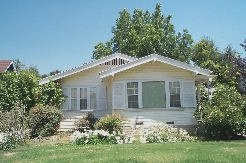
\includegraphics[width=0.45\textwidth]{./Figures/calhouse_237/9048-resultado.jpg}
    }
%        \caption{Imagen Original. $\mathscr{H_Y}=0.207231$. $SSIM_R=1$. $SSIM_G=1$. $SSIM_B=1$}
\end{subfigure}
    ~ %add desired spacing between images. e. g. ~. \quad. \qquad. \hfill etc. 
      %(or a blank line to force the subfigure onto a new line)
      \begin{subfigure}[ID=1]{
      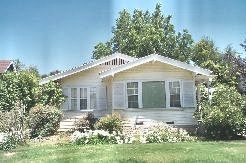
\includegraphics[width=0.45\textwidth]{./Figures/calhouse_237/9090-resultado.jpg}   
      }
    %\begin{subfigure}[t]{0.45\textwidth}
%        \caption{Enhanced Image. $\mathscr{H_Y}=0.611275$. $SSIM_R=0.00897331$. $SSIM_G=0.00823064$. $SSIM_B=0.00851013$}
\end{subfigure}
    ~ %add desired spacing between images. e. g. ~. \quad. \qquad. \hfill etc. 
    %(or a blank line to force the subfigure onto a new line)
    \begin{subfigure}[ID=23]{
    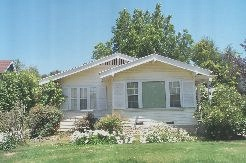
\includegraphics[width=0.45\textwidth]{./Figures/calhouse_237/9095-resultado.jpg}
    }
    % \begin{subfigure}[t]{0.45\textwidth}
%        \caption{Enhanced Image.  $\mathscr{H_Y}=0.0350595$. $SSIM_R=0.416776$. $SSIM_G=0.403636$. $SSIM_B=0.417654$}
\end{subfigure} 
\begin{subfigure}[ID=24]{
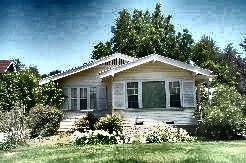
\includegraphics[width=0.45\textwidth]{./Figures/calhouse_237/9162-resultado.jpg}
}
    % \begin{subfigure}[t]{0.45\textwidth}
        %\caption{Enhanced Image using \cite{morepso}. $\mathscr{H_Y}=0.788927$. $SSIM_R=0.000204143$. $SSIM_G=0.0000526475$. $SSIM_B=0.0000518143$}
        % \label{fig:calhouse23129}
        \end{subfigure}
    ~ %add desired spacing between images. e. g. ~. \quad. \qquad. \hfill etc. 
    %(or a blank line to force the subfigure onto a new line)
    \begin{subfigure}[ID=56]{
    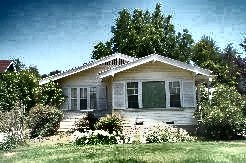
\includegraphics[width=0.45\textwidth]{./Figures/calhouse_237/9175-resultado.jpg}
    }
    % \begin{subfigure}[t]{0.45\textwidth}
%        \caption{Enhanced Image.  $\mathscr{H_Y}=0.0350595$. $SSIM_R=0.416776$. $SSIM_G=0.403636$. $SSIM_B=0.417654$}
% \label{fig:calhouse231102}
\end{subfigure} 
\begin{subfigure}[Imagen Original]{
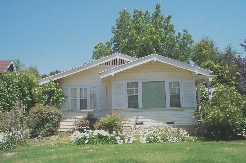
\includegraphics[width=0.45\textwidth]{./Figures/calhouse_237/calhouse_237.jpg}
}
    % \begin{subfigure}[t]{0.45\textwidth}
        %\caption{Enhanced Image using \cite{morepso}. $\mathscr{H_Y}=0.788927$. $SSIM_R=0.000204143$. $SSIM_G=0.0000526475$. $SSIM_B=0.0000518143$}
        % \label{fig:calhouse233orig}
        \end{subfigure}
        \caption{Imágenes visualmente relevantes obtenidas mediante $CMOPSO-CLAHE$. Las variables y decisión y métricas de las imágenes se muestran en la tabla \ref{tab:calhouse_237}.}
        \label{fig:anexocalhouse237}
        \end{figure}

        \begin{figure}[H]
        \centering
        %\begin{subfigure}[Gráfica de Frente Pareto para las soluciones no dominadas de \texttt{calhouse_231.jpg}]{
        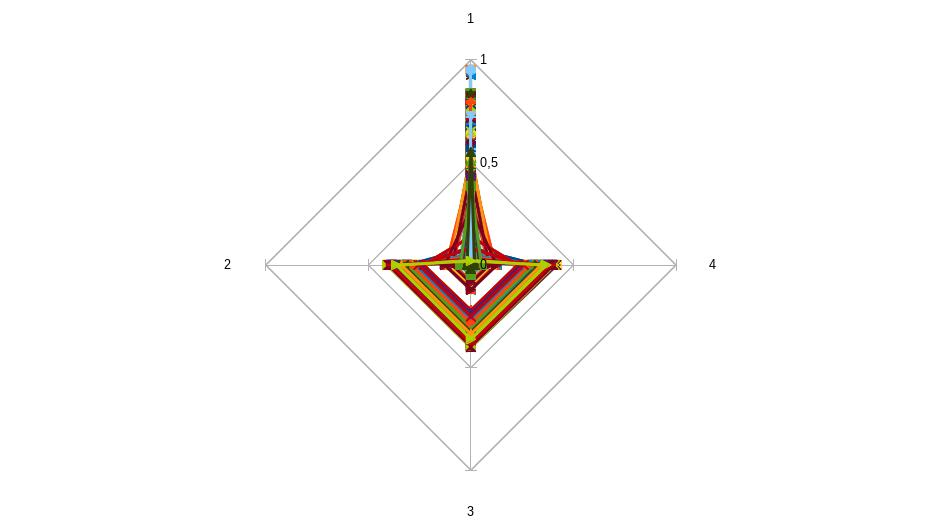
\includegraphics[width=\textwidth]{./Figures/calhouse_237/calhouse_237_2.jpg}
        %}
        %\end{subfigure}
        \caption{Frente pareto que contrasta los objetivos de las soluciones no dominadas. para los resultados de imágenes que se muestran en la tabla \ref{tab:calhouse_237}.}
        \label{fig:calhouse2372fp}
        \end{figure}        
% \begin{table}[H]
% \centering
% \caption{Promedios de los tiempos de ejecución de algoritmo HE para las imágenes en escala de grises.}
% \label{tabla22}
% \begin{tabular}{|c|c|}
% \hline
% \begin{tabular}[c]{@{}c@{}}Nº de \\ ejecución\end{tabular} & \begin{tabular}[c]{@{}c@{}}t\\ (ms)\end{tabular} \\ \hline
% 1                                                          & 1.145                                            \\
% 2                                                          & 0.945                                            \\
% 3                                                          & 0.97                                             \\
% 4                                                          & 0.925                                            \\
% 5                                                          & 0.95                                             \\ \hline
% Promedio                                                   & \textbf{0.987}                                   \\ \hline
% \end{tabular}
% \end{table}


% En la Tabla \ref{tabla23} se muestran los promedios de los tiempos de ejecución del algoritmo MMCE para las imágenes en escala de grises.

% % Please add the following required packages to your document preamble:
% % \usepackage{multirow}
% \begin{table}[H]
% 	\centering
% 	\caption{Promedios de los tiempos de ejecución del algoritmo MMCE para las imágenes en escala de grises.}
% 	\label{tabla23}
% 	\begin{tabular}{|c|c|c|c|c|c|c|}
% 		\hline
% 		\multirow{2}{*}{Iter. (n)} & \multicolumn{5}{c|}{Nº de ejeciciones para el algoritmo MMCE} & \multirow{2}{*}{\begin{tabular}[c]{@{}c@{}}Promedios\\ t(ms)\end{tabular}} \\ \cline{2-6}
% 		& 1           & 2          & 3         & 4         & 5          &                                                                            \\ \hline
% 		1                          & 64.265      & 62.625     & 61.61     & 62.285    & 62.295     & \textbf{62.616}                                                            \\
% 		2                          & 165.805     & 171.24     & 169.655   & 170.515   & 170.295    & \textbf{169.502}                                                           \\
% 		3                          & 327.975     & 334.19     & 334.75    & 332.045   & 333.275    & \textbf{332.447}                                                           \\
% 		4                          & 564.035     & 574.15     & 571.185   & 573.45    & 568.735    & \textbf{570.311}                                                           \\
% 		5                          & 975.845     & 972.035    & 979.205   & 968.975   & 986.805    & \textbf{976.573}                                                           \\
% 		6                          & 1454.415    & 1471.145   & 1449.78   & 1452.97   & 1463.74    & \textbf{1458.41}                                                           \\
% 		7                          & 2037.11     & 2032.775   & 2041.54   & 2029.07   & 2038.735   & \textbf{2035.846}                                                          \\ \hline
% 	\end{tabular}
% \end{table}


% En la Tabla \ref{tabla24} se muestran los promedios de los tiempos de ejecución del algoritmo propuesto para las imágenes en escala de grises.

% % Please add the following required packages to your document preamble:
% % \usepackage{multirow}
% \begin{table}[H]
% 	\centering
% 	\caption{Promedios de los tiempos de ejecución del algoritmo propuesto para las imágenes en escala de grises.}
% 	\label{tabla24}
% 	\begin{tabular}{|c|c|c|c|c|c|c|}
% 		\hline
% 		\multirow{2}{*}{Iter. (n)} & \multicolumn{5}{c|}{Nº de ejeciciones para el algoritmo propuesto} & \multirow{2}{*}{\begin{tabular}[c]{@{}c@{}}Promedios \\ t(ms)\end{tabular}} \\ \cline{2-6}
% 		& 1            & 2           & 3           & 4          & 5          &                                                                             \\ \hline
% 		1                          & 62.105       & 63.055      & 61.99       & 62.445     & 62.955     & 62.51                                                                       \\
% 		2                          & 166.74       & 169.645     & 168.34      & 168.435    & 169.34     & 168.5                                                                       \\
% 		3                          & 327.175      & 332.58      & 331.765     & 332.755    & 331.52     & 331.159                                                                     \\
% 		4                          & 565.245      & 576.84      & 574.47      & 573.6      & 572.15     & 572.461                                                                     \\
% 		5                          & 976.57       & 973.22      & 968.35      & 970.245    & 975.26     & 972.729                                                                     \\
% 		6                          & 1463.175     & 1474.82     & 1458.765    & 1459.83    & 1470.06    & 1465.33                                                                     \\
% 		7                          & 2047.435     & 2040.82     & 2041.915    & 2039.95    & 2044.16    & 2042.856                                                                    \\ \hline
% 	\end{tabular}
% \end{table}

